\documentclass[11pt]{article}

\usepackage[margin=1in]{geometry}
\usepackage{booktabs}
\usepackage{graphicx}
\usepackage[section]{placeins}
\usepackage{hyperref}
\hypersetup{colorlinks=true, linkcolor=blue!50!black,
citecolor=green!35!black, urlcolor=cyan!40!black}
\usepackage{natbib}
\usepackage{array}
\usepackage{microtype}
\usepackage{amsmath}
\usepackage{amssymb}
\usepackage{amsthm}
\usepackage{pgfplots}
\pgfplotsset{compat=1.17}
\definecolor{vfblue}{HTML}{0072B2}
\definecolor{rollver}{HTML}{D55E00}
\definecolor{mutedink}{HTML}{555555}
\definecolor{surteal}{HTML}{009E73}
\definecolor{flatpink}{HTML}{CC79A7}

\newtheorem{theorem}{Theorem}
\newtheorem{lemma}{Lemma}
\newtheorem{proposition}{Proposition}
\newtheorem{assumption}{Assumption}
\newtheorem{remark}{Remark}
\newtheorem{hypothesis}{Hypothesis}
\newtheorem{corollary}{Corollary}

\setlength{\emergencystretch}{3em}

\newcommand{\Vstar}{V^{\star}}
\newcommand{\pol}{\pi_{\lambda}}

\title{Certified-Gap Dual-Price Policies for Real-Time Truckload Bid
Acceptance with Relocating, Clock-Constrained
Resources\thanks{Evaluation artifact: FreightBidBench
(contracts \texttt{freightbidbench-v0.4-dev} and
\texttt{-v0.4.1}, release tag \texttt{v0.4.2});
\url{https://github.com/aswincsekar/freightbidbench}. All values
reproduce per Appendix~\ref{sec:repro}.}}
\author{Aswin Chandrasekaran \\ Bubba AI \\ \texttt{aswin@bubba.ai}}
\date{August 2026}

\begin{document}
\maketitle

\begin{abstract}
A truckload carrier must accept or reject each load tender within
seconds, under fleet state, hours-of-service clocks, and appointment
windows. We model this as a weakly coupled dynamic program whose
resources relocate and carry clocks --- service capability is a
controlled state variable --- a combination outside occupancy-based
reusable-resource models and the stateless relocating-resource
pricing line.

We build a real-time dual-price policy from the same Lagrangian
relaxation that gives the problem's upper bound, so every run can
report a \emph{certified optimality gap}. Three results. The certificate is
valid for any duals, any permissive discretization, and any surrogate
quality (Theorem~1). In the subcritical fluid regime --- analyzed in a
grid-aligned hourly idealization of the model --- the policy's same-time
spatial-gradient rule is exactly fluid complementary slackness, a
lane-priced, soft-margin variant is asymptotically optimal with an
asymptotically tight certificate, and the fitted prices are portable
across sample paths by linear-programming basis stability (Theorem~2;
both convergence statements hold as predicted on an
assumption-matched synthetic family run through the paper's own
pipeline).
Certificates also have limits: a three-truck kernel with exact
rational primal--dual certificates and a replication lemma shows
per-resource Lagrangian slack bounded away from zero at arbitrarily
large fleet sizes (Theorem~3).

On a public closed-loop benchmark with thirty paired seeds, the policy
--- one offline dual solve, no rollout labels --- beats a
rollout-trained surrogate on two of three scenarios (tight:
$+2.1$~pp, 95\% CI $[+0.5, +3.7]$; mild: $+3.5$~pp), with no
statistically detectable difference on the third ($-0.9$~pp,
$[-3.1, +1.4]$), deciding in 0.02--0.04\,ms --- roughly three
orders of magnitude below the rollout teacher's 48--112\,ms, a
separation large enough to survive the cross-host latency caveat of
the experiments section. A re-solving deterministic-LP baseline,
its cadence tuned on training streams, is the stronger profit
baseline on the two stress scenarios and weaker on the third, while
swinging up to 29 points with its cadence; the certifier is
policy-agnostic and certifies it too. The dual policy's contribution
is therefore not profit dominance over re-solving: it is a static,
fit-once policy with a theoretical characterization --- fluid
consistency and certificate tightness in the subcritical regime ---
inside a framework whose ex-post, per-instance certifier prices every
policy on the same scale. Its certificates are stable
across ten bounded instances per scenario --- certified $\geq$
57.6--60.1\% of the hindsight optimum, within 2.7--6.0 points of what
the roughly $1000\times$-slower teacher itself certifies
(62.8--63.6\%; latency hosts differ); its fitted prices are interchangeable across five
independent training streams (tight scenario). Across sixty micro-instances where we compute the joint optimum
exactly --- half by a randomized-window, ex-ante-placement design with
service chains up to length four --- an integral optimal solution is
found on 56
and, pooled, at least $85\%$ of the certificate gap is policy loss,
not relaxation slack.
\end{abstract}

\section{Introduction}
\label{sec:intro}

Truckload carriers and brokers answer a stream of load tenders in real
time. Each acceptance consumes a truck. The truck's future usefulness
depends on where the load delivers it and how much drive and duty time
its driver has left. Each rejection preserves options whose value
depends on demand that has not arrived yet. A widely used family of
future-aware methods --- and the strongest baseline in the public
benchmark below --- is finite-lookahead Monte Carlo rollout
\citep{bertsekas1997rollout,goodson2017rollout}; dynamic truckload
acceptance and fleet-management formulations go back further
(\S\ref{sec:related}). Rollout is
accurate, but it costs tens to hundreds of milliseconds per decision
and scales poorly with fleet size. The benchmark release preceding this
paper, FreightBidBench v0.3 \citep{chandrasekaran2026freightbidbench},
made the problem reproducible: public calibration, explicit
feasibility, versioned contracts, and hindsight upper bounds. Its best
latency-aware method, a surrogate-to-rollout cascade, recovers about
$98\%$ of rollout profit. But the cascade inherits rollout's cost on
escalated decisions, and it says nothing about distance from
\emph{optimal}.

This paper asks the harder question the bounds make precise:
\textbf{how close to optimal can a real-time policy be, and can that
closeness be certified per instance?} We use one object twice.

The logic fits in a paragraph. The only constraint coupling the trucks
is that each load can be served by at most one of them. Dualize it,
and each load's slot acquires a price $\lambda_t$; each truck then
solves its own small planning problem against those prices, free of
the other trucks. Summing the per-truck values (plus the prices) can
only overcount the true optimum --- that sum is the upper bound. But
the same solution also says what a slot costs and what standing in
each market is worth. We compress both into two small tables, fitted
once, offline. The policy is then a lookup: accept a load exactly when
its profit, plus the value of ending up somewhere new, clears the
slot price. No rollout simulation, training labels, or online
optimization ever enters the decision loop. The certificate uses the
same relaxation in a second, separate role: an \emph{ex-post},
per-instance bound computation on the realized stream --- optional,
offline, and policy-agnostic (it certifies any feasible policy, not
just ours) --- so every reported run ships with realized policy value
against realized bound.

Pairing a Lagrangian policy with its bound is the standard playbook of
weakly coupled dynamic programs. The contribution here is the model in
which we make it work, the form of the policy, and the two-sided theory
of the certificate:

\begin{enumerate}
\item \textbf{Model (\S\ref{sec:model}).} Resources whose \emph{service
  capability is a controlled state variable}: feasibility depends on
  location and HOS clocks, service relocates the truck, and rest
  restores the clocks. The adjacent literatures --- weakly coupled
  DPs, online reusable resources, dual mirror descent, and, closest,
  Lagrangian pricing of relocating resources
  \citep{balseirobrownchen2021relocating} --- each lack at
  least one of these ingredients (\S\ref{sec:related}).
\item \textbf{Policy and certificate
  (\S\ref{sec:policy}--\ref{sec:certs}).} A dual-price policy whose
  relocation term is a \emph{same-time spatial gradient}, and
  Theorem~\ref{thm:cert}: the certificate is valid for any duals, any
  permissive discretization, and any surrogate quality. The design
  rule is \emph{duals price time, gradients price place}; the naive
  rule that charges time twice collapses to 24--30\% of rollout
  across the full thirty-pair design (Lemma~\ref{lem:doublecount},
  Hypothesis~\ref{hyp:doubleshade}).
\item \textbf{Fluid theory (\S\ref{sec:fluid}).} In the subcritical
  regime the gradient rule is exactly fluid complementary slackness,
  and a lane-priced, soft-margin variant of the policy is
  asymptotically optimal with an asymptotically tight certificate
  (Theorem~\ref{thm:fluid}, Corollary~\ref{cor:tight}; both stated
  for a grid-aligned hourly idealization of the model,
  Remark~\ref{rem:gridgap}). The same
  basis-stability argument explains why fitted prices are
  \emph{portable across independent training realizations}, and
  predicts where portability fails.
\item \textbf{Limits (\S\ref{sec:limits}).} Certificates cannot
  promise everything: a three-truck kernel with exact rational primal
  and dual certificates shows per-resource Lagrangian slack can stay
  bounded away from zero at arbitrarily large fleet sizes
  (Theorem~\ref{thm:kernel}). Such kernels were rare under our
  particular random instance sampler (${\sim}0.03\%$ of draws);
  whether they matter at benchmark scale is an attribution question we
  treat empirically.
\item \textbf{Evidence (\S\ref{sec:experiments}).} On thirty paired
  seeds the policy beats a rollout-trained surrogate on two of three
  scenarios, with no statistically detectable difference on the
  third, at roughly $1000\times$ lower latency than rollout
  (latencies timed on different hosts; the ratio is indicative); a cadence-tuned re-solving LP baseline earns more
  profit on the stress scenarios (and less on mild, swinging up to
  29~pp with its cadence) --- the dual policy's distinct
  offer is a static, fit-once policy with a fluid-regime
  characterization, and the certifier is an ex-post, per-instance
  computation, policy-agnostic by design, certifying the DLP and
  rollout as well; Theorem~\ref{thm:fluid}'s convergence
  predictions hold on an assumption-matched synthetic family run
  through the paper's own pipeline, production shrinkage included
  (certified fraction $70.2 \to 99.8\%$, per-truck gap
  $\$819 \to \$6.6$ over $K = 48$--$768$, thirty train/eval pairs
  per size); its (tight-scenario)
  fitted prices are interchangeable across five independent training
  realizations; and on micro-instances where the joint optimum is
  exactly computable --- including a randomized-window, ex-ante
  placement design with service chains up to length four --- the
  certificate gap is overwhelmingly policy loss, not relaxation
  slack.
\end{enumerate}

\subsection{Related work}
\label{sec:related}

\paragraph{Weakly coupled DPs and bid prices.} Bid-price control goes
back to \citet{talluri1998bidprice}, and fluid policies are
asymptotically optimal in classical network revenue management
\citep{gallego1997network}. Dynamic bid prices from value
approximations originate with \citet{adelman2007dynamic};
Lagrangian decompositions of weakly coupled DPs with policy-plus-bound
pairing are standard since \citet{hawkins2003lagrangian},
\citet{adelman2008relaxations}, and \citet{topaloglu2009lagrangian}, who
reports bounds and policy values on the same network revenue-management
instances. Our Theorem~\ref{thm:cert} inherits this mechanism; the
extension is the resource model (state-dependent participation,
controlled relocation) and the explicit certificate framing at
sub-millisecond decision latency. \citet{brownzhang2023strength} bound
the ALP--Lagrangian gap by $O(1)$ constants under conditions on linking
constraints that state-dependence violates; Theorem~\ref{thm:kernel}
constructs instances with exactly the behavior their conditions
exclude --- in the natural freight scaling, constraints number
$\propto K$ and participation is state-dependent. (The benchmark's
growing \emph{reported} certificate gaps in Table~\ref{tab:scaling}
are consistent with that mechanism but confounded with dual
convergence; \S\ref{sec:experiments} keeps the attribution open.)

\paragraph{Relocating and reusable resources.} The closest prior
work is \citet{balseirobrownchen2021relocating}, who price relocating
resources on a hub-and-spoke network: one Lagrangian relaxation
yields both a dynamic pricing policy and an upper bound, and the
policy's loss is $O(\ln n / n)$ in a supply-constrained large-network
regime (spokes and resources scaling together). That is the template
for policy-plus-bound pairing under relocation, and our mechanism
parallels it. The differences define this paper's claim: (i) their
resources carry no internal state beyond location --- participation
is availability-only --- whereas our trucks carry HOS clocks and
window feasibility, so service capability is a controlled state
variable; (ii) their control is per-request pricing, ours is
accept/reject under exogenous prices at a hard latency budget; (iii)
their guarantee is asymptotic in a scaling regime, whereas our
certificate is ex-post on each realized instance, valid for any duals
at any scale (Theorem~\ref{thm:cert}), with tightness proved only in
the subcritical regime (Theorem~\ref{thm:fluid}) and impossible in
general (Theorem~\ref{thm:kernel}); (iv) the asymptotic regimes
differ --- they scale network size with supply, we scale fleet and
demand on fixed lane geometry. \citet{zhangcheung2022reusable}
and the nonstationary extension \citet{zhangcheung2025nonstationary}
allocate units that occupy and \emph{return unchanged}; feasibility
is availability-only. A truck returns elsewhere with depleted clocks.
The distinction is not cosmetic, but the honest statement is
narrower than ``relocation breaks integrality'':
\citet{brownzhang2023strength} place price-directed control of
relocating resources among the models satisfying their zero-gap
structural conditions, so relocation alone does not produce
Lagrangian slack --- rather, clock- and state-dependent participation
creates chain-conflict structures absent from standard
price-directed relocating-resource models, and
Theorem~\ref{thm:kernel}'s kernel exhibits exactly such a structure
(\S\ref{sec:limits}); the same structure is what the same-time
gradient prices (\S\ref{sec:fluid}). The recent reusable-resource
frontier sharpens the frame: stock-dependent two-price policies
attain the optimal pricing loss \citep{balseiromazhang2025twoprices},
online allocation admits an asymptotically optimal competitive ratio
\citep{goyaliyengarudwani2025reusable}, and overloaded networks admit
logarithmic regret \citep{xiegurvichkucukyavuz2025logregret}. None of
these carries clock-dependent participation, which is where our model
lives --- and they mark where our theory is weaker: outside the
subcritical regime we offer a certificate, not a competitive ratio or
regret guarantee.

\paragraph{Online allocation with dual updates.} \citet{balseiro2020dual}
attain optimal $O(\sqrt{T})$ regret with per-request dual mirror descent
for consumable budgets, motivated by the same latency constraints. We
deliberately make no regret-rate claim --- rates are a settled
literature --- and instead fix prices offline (portable by
Lemma~\ref{lem:stability}), leaving the online variant to future work.
A related alternative is re-solving a deterministic LP at each decision
epoch, which achieves excellent regret in network revenue management;
per-decision solves conflict with microsecond latency at growing
instance sizes, so we implement the periodically re-solving variant
as a baseline instead (\texttt{dlp\_resolve},
\S\ref{sec:experiments}); with its cadence tuned on training streams
it out-earns the dual policy on two of three scenarios, and the
comparison we draw is on certificates and fit-once deployment, not
profit dominance. Re-solving is subtle in theory: conventional periodic
re-solving does not by itself improve the DLP's asymptotic loss
\citep{jasinkumar2013lp}, while carefully scheduled variants attain
uniformly bounded loss \citep{bumpensantiwang2020resolving}; ours is
the conventional periodic variant.

\paragraph{Dynamic truckload acceptance.} The accept/reject problem
itself has a direct lineage. \citet{kim2004dynamic} propose and
simulate dynamic acceptance/rejection policies for large truckload
fleets with time windows; \citet{yang2004realtime} compare
rolling-horizon strategies --- including repeated reoptimization ---
for real-time multivehicle truckload pickup and delivery;
\citet{topaloglupowell2007pricing} incorporate
pricing into stochastic dynamic fleet management through ADP value
approximations. These lines optimize or approximate the same class of
decisions; none reports per-instance optimality certificates, and
their evaluations use proprietary or single-study instances rather
than a versioned public benchmark --- the two gaps this paper and its
companion \citep{chandrasekaran2026freightbidbench} target.

\paragraph{Fleet ADP.} Industrial-scale approximate dynamic programming
for truckload fleets \citep{simao2009adp,powell2007stochastic} produced
marginal values of driver states as model outputs, aimed at calibration
rather than optimality certification; no per-instance gap reporting
appears in this line.

\paragraph{Compute-aware deferral.} Value-of-computation metareasoning
for Monte Carlo search \citep{sezener2020voc} has not been applied to
operational dispatch; the benchmark's cascade and this paper's policy
make the freight instantiation available, and we leave a learned
deferral rule to future work.

\section{Model}
\label{sec:model}

\subsection{Resources, requests, and controlled relocation}

Time runs on $[0, T]$. A fleet of $K$ resources (trucks) has
states $x_k = (m_k, \tau_k, h_k, d_k) \in \mathcal{X}$: market $m$ in a
finite set $\mathcal{M}$, next-available time $\tau$, and remaining
drive/duty clocks $(h, d)$. Requests (load tenders)
$\ell_1, \dots, \ell_N$ arrive at times $t_1 \leq \dots \leq t_N$
and are processed in this (index) order; in the idealized hourly model
of \S\ref{sec:fluid}, all of an epoch's requests share its timestamp
and are processed sequentially in index order after the epoch's
completions release; request
$\ell$ carries origin $o(\ell)$, destination $\delta(\ell)$, and the
price/cost/window attributes of the benchmark. Three primitives
distinguish the model from occupancy-based reusable resources:

\begin{itemize}
\item \textbf{State-dependent feasibility.} A deterministic map
  $f(x, \ell) \in \{0, 1\}$ gates service: $f = 1$ only if the resource
  is in the origin market, can reach the pickup inside its appointment
  window, and admits an HOS-feasible schedule through delivery.
\item \textbf{Controlled relocation.} Serving executes
  $x \leftarrow S(x, \ell)$: the market becomes $\delta(\ell)$, the
  next-available time advances by the service duration including
  inserted rests, and the clocks are updated by the drive/duty consumed.
  The resource does not return to its prior pool state.
\item \textbf{Autonomous renewal.} Idle resources renew clocks by
  resting (11/14/10 in the benchmark), so service capability regenerates
  in a state-dependent way.
\end{itemize}

\subsection{Joint control problem}

At each arrival $t$ the controller observes $(x_1, \dots, x_K, \ell_t)$
and chooses $a_t \in \{0, 1, \dots, K\}$ (reject, or assign to a
feasible resource). Writing $a^{(k)}_t = \mathbf{1}\{a_t = k\}$, the
joint constraint is $\sum_k a^{(k)}_t \leq 1$. Rewards follow the
benchmark: realized profit $r(x_k, \ell_t)$ on feasible accepts, a
service-failure penalty on infeasible attempts (excluded under
$f$-gated policies), and terminal fleet value
$\Phi = \omega \sum_k V(m_k(T))$. $\Vstar(\xi)$ denotes the optimum on
realized scenario $\xi$.

\subsection{Lagrangian per-resource decomposition}
\label{sec:lagrangian}

Dualizing the joint constraint with prices
$\lambda = (\lambda_t) \geq 0$,
\begin{equation}
  L(\lambda; \xi) \;=\; \sum_t \lambda_t
  \;+\; \sum_k V^k_{\lambda}(x_k(0); \xi),
  \label{eq:lag}
\end{equation}
where $V^k_{\lambda}$ is resource $k$'s optimal value in its own sub-MDP
with per-service reward $r(x, \ell_t) - \lambda_t$, retaining $f$, $S$,
and renewal. Weak duality gives $\Vstar(\xi) \leq L(\lambda; \xi)$
pointwise for every $\lambda \geq 0$ (see also the
information-relaxation view of \citealp{brown2010information}). The benchmark computes $L$ by
bucketed forward enumeration over an \emph{augmented} per-resource
system that additionally grants a voluntary timed rest
(\texttt{RESET\_HOURS} of wall-clock, clocks renewed) before any
service. The augmentation is what makes the bucketing sound: rounding
clocks down is \emph{not} permissive on its own, because mandatory
rests renew clocks --- a higher-usage state can be strictly more
valuable when service triggers a reset --- but with voluntary rest
available, a lower-usage state reproduces any renewed-clock state a
higher-usage plan reaches, at no later a completion time, so the
snapped bucket corner dominates every state in its bucket. Adding
actions can only raise per-resource optima, so $L$ computed on the
augmented system still upper-bounds the true $L$, hence $\Vstar$
(a one-truck counterexample without the augmentation, and randomized
one-truck audits against the exact joint DP, ship in the test suite).
Per-resource solves
parallelize (standard-library multiprocessing; bit-identical to serial).

\section{The Dual-Price Policy}
\label{sec:policy}

The relaxation's solution is rich --- one price per realized load,
one value function per truck --- but a deployable policy cannot carry
per-load objects into unseen streams. This section compresses the
solution into two small tables and reads the acceptance rule off
them.

\subsection{Price and value surrogates}
\label{sec:surrogates}

Fix any duals $\lambda \geq 0$ (in practice a few tens of subgradient
iterates on one training scenario). Two aggregated objects are fitted
offline:

\begin{itemize}
\item \textbf{A price surface}: the mean dual of loads, fitted either
  by origin market and hour-of-day
  ($\hat{\lambda} : \mathcal{M} \times [0, 24) \to \mathbb{R}_{\geq 0}$,
  the deployed table --- lower variance, uses shrinkage) or at
  lane--hour granularity (the variant analyzed in
  \S\ref{sec:fluid}; Lemma~\ref{lem:stability} identifies its limit as
  the fluid rent $\mathbb{E}[(r - \theta_{\ell h})_+]$, and
  Remark~\ref{rem:granularity} quantifies the gap between the two).
\item \textbf{An aggregated value-to-go}
  $\widehat{W} : \mathcal{M} \times [0, T] \to \mathbb{R}$: the backward
  recursion on the (market, hour) grid over the realized train stream
  with dual-netted rewards, $\widehat{W}(m, T) = \omega V(m)$ and
  \begin{equation}
    \widehat{W}(m, t) = \max\Bigl( \widehat{W}(m, t{+}1),\;
    \max_{\ell:\, t_\ell = t,\, o(\ell) = m}
    \bigl[ \bar{r}(\ell) - \lambda_{t_\ell}
    + \widehat{W}(\delta(\ell), t + \tau(\ell)) \bigr] \Bigr).
    \label{eq:wrec}
  \end{equation}
  Here $\bar{r}(\ell)$ is the \emph{net} realized profit of the
  feasibility layer (linehaul revenue minus direct, deadhead, and
  expected yard-delay costs) and $\tau(\ell)$ is the rest-inclusive
  completion advance of a fresh in-market truck's planned schedule ---
  the same reward and transition the Lagrangian sub-MDP uses, so
  $\widehat{W}$ approximates that sub-MDP's value on the aggregated
  state (\path{scripts/fit_value_togo.py}).
\end{itemize}

\subsection{Policy}
\label{sec:policydef}

The policy makes three moves at each arrival $\ell$ at time $t$.

\emph{Step 1: pick the truck.} Among feasible trucks, take the one
with the best realized profit:
\begin{equation}
  k^{\star} \in \arg\max_{k :\, f(x_k, \ell) = 1} r(x_k, \ell).
\end{equation}

\emph{Step 2: price the decision.} Compute the relocation gain first.
It is the value of standing at the destination instead of the origin,
compared at the same time $t + \tau(\ell)$ --- the chosen truck's
actual schedule completion, rests included:
\begin{equation}
  g(\ell, t) \;=\; \widehat{W}\bigl(\delta(\ell), t + \tau(\ell)\bigr)
  \;-\; \widehat{W}\bigl(o(\ell), t + \tau(\ell)\bigr).
  \label{eq:gradient}
\end{equation}
Then start from the profit, subtract the price of the slot, and add the
relocation gain:
\begin{equation}
  \mathrm{score} \;=\; r(x_{k^{\star}}, \ell)
  \;-\; \hat{\lambda}(o(\ell), t) \;+\; g(\ell, t).
  \label{eq:policy}
\end{equation}

\emph{Step 3: decide.} Accept with $k^{\star}$ iff
$\mathrm{score} \geq 0$.

We call $g$ the \textbf{same-time spatial gradient}. The busy-time
opportunity cost is priced once, by $\hat{\lambda}$; $g$ prices only
the change of place. Each decision costs a feasibility probe over
origin-market resources plus two table lookups. Measured latency is
0.02--0.12\,ms across fleet sizes 35--140, versus 32--159\,ms for
rollout. The advantage widens with fleet size.

\section{Certified Gaps}
\label{sec:certs}

The policy came from a relaxation; this section states what that
buys. The theorem is deliberately unconditional: nothing about the
quality of the duals, the discretization, or the fitted tables is
assumed. Validity is structural --- errors anywhere degrade the
policy or loosen the bound, but they can never make the certificate
lie.

\begin{theorem}[Certified optimality gap]
\label{thm:cert}
Let $\lambda \geq 0$ be arbitrary and $\pi$ any feasible policy. On
every realized scenario $\xi$,
$V^{\pi}(\xi) \leq \Vstar(\xi) \leq L(\lambda; \xi)$, hence the
observable $\mathrm{gap}(\xi) := L(\lambda; \xi) - V^{\pi}(\xi)$
upper-bounds the true suboptimality $\Vstar(\xi) - V^{\pi}(\xi)$. The
certificate remains valid for any $\lambda$, any per-resource
discretization with the permissive-corner property (each bucket's
representative dominates every state in its bucket \emph{within the
solver's --- possibly augmented --- action system}; the benchmark
achieves this with a voluntary-rest action, \S\ref{sec:lagrangian}),
and any quality of
$\hat{\lambda}, \widehat{W}$ --- surrogate error degrades policy value
(widening the reported gap) but never invalidates the certificate.
\end{theorem}

\begin{proof}
We argue in four short steps.

\emph{Step 1.} $V^{\pi}(\xi) \leq \Vstar(\xi)$. The policy $\pi$
is feasible, and $\Vstar(\xi)$ is by definition the best value any
feasible policy attains on $\xi$.

\emph{Step 2.} $\Vstar(\xi) \leq L(\lambda; \xi)$. This is weak
duality for the dualized joint constraint (\S\ref{sec:lagrangian}),
and it holds pointwise in $\xi$ for every $\lambda \geq 0$.

\emph{Step 3.} Subtract $V^{\pi}(\xi)$ from both sides of Step~2:
\[
  \Vstar(\xi) - V^{\pi}(\xi) \;\leq\; L(\lambda; \xi) - V^{\pi}(\xi)
  \;=\; \mathrm{gap}(\xi).
\]

\emph{Step 4.} The invariances. The certificate uses two ingredients
only: an upper bound computed from $(\lambda, \xi)$, and the realized
value of a feasible policy. Neither ingredient depends on how $\lambda$
was chosen, on the discretization (which can only enlarge the bound,
by the permissive-corner property), or on the quality of
$\hat{\lambda}, \widehat{W}$ (which affect only which feasible policy
we happen to run).
\end{proof}

\begin{proposition}[Exactness]
\label{prop:exact}
If $\lambda^{\star}$ minimizes $L(\cdot\,; \xi)$ and the per-resource
optimizers jointly satisfy primal feasibility and complementary
slackness, the assembled plan is optimal and the certificate is tight.
\end{proposition}

In practice a residual contested set (${\sim}1$--$2\%$ of loads) keeps
the certificate strictly positive.

\begin{lemma}[Continuation decomposition]
\label{lem:doublecount}
At a decision $(\ell, t)$ with $t' = t + \tau(\ell)$, define
\[
  D_{\mathrm{time}} \;=\; \widehat{W}(o, t) - \widehat{W}(o, t'),
  \qquad
  D_{\mathrm{place}} \;=\; \widehat{W}(\delta, t') - \widehat{W}(o, t').
\]
Then (i) the naive continuation splits exactly,
$\widehat{W}(\delta, t') - \widehat{W}(o, t)
= D_{\mathrm{place}} - D_{\mathrm{time}}$; and (ii)
$D_{\mathrm{time}} \geq 0$ is the \emph{window option value}: the
incremental value, under recursion~\eqref{eq:wrec}, of the resource
being dispatchable at $o$ during $[t, t')$ rather than only from $t'$
(including any post-window continuation difference of the chains it
enables).
\end{lemma}

\begin{proof}
\emph{Step 1.} Part (i) is a one-line check: add and subtract
$\widehat{W}(o, t')$.

\emph{Step 2.} For (ii): the wait branch of \eqref{eq:wrec} makes
$\widehat{W}(m, \cdot)$ non-increasing, so $D_{\mathrm{time}} \geq 0$.
Unrolling the max branches from $t$ until the first branch that waits
past $t'$ shows $\widehat{W}(o, t) = \max\bigl( \widehat{W}(o, t'),\;
\max\,\{\text{dual-netted value of chains first dispatched in }
[t, t')\} \bigr)$, where each chain's value includes its full
continuation beyond the window. The difference of the two maxima is
exactly the option value of the window.
\end{proof}

\begin{hypothesis}[Double shading]
\label{hyp:doubleshade}
On contested streams the fitted price $\hat{\lambda}$ already reflects
the rent of the busy slots (its limit under
Lemma~\ref{lem:stability} is the per-slot rent
$\mathbb{E}[(r - \theta)_+]$), so a rule that additionally subtracts
$D_{\mathrm{time}}$ shades the same opportunity twice and
under-accepts. The same-time gradient $g = D_{\mathrm{place}}$ avoids
the second charge by construction.
\end{hypothesis}

We state this as a hypothesis, not a theorem: $\lambda_t$ is formally
the dual of the one-truck-per-load coupling constraint, and
identifying it with a busy-time capacity price is exact only in the
fluid limit (where Lemma~\ref{lem:stability} gives the rent identity
and, by Remark~\ref{rem:honest}, $D_{\mathrm{time}}$ itself vanishes
so the two rules coincide). The hypothesis earns its keep at finite
$K$ on contested streams, where its prediction is dramatic and
confirmed: the naive rule collapses to 24.4--29.9\% of rollout
profit across the full thirty-pair design while the gradient rule
attains 90.2--101.8\% (\S\ref{sec:experiments}). \emph{Duals price time; gradients price
place} is the design heuristic this supports.

\section{Fluid Consistency in the Subcritical Regime}
\label{sec:fluid}

The certificate of \S\ref{sec:certs} is always valid but says nothing
about tightness. This section identifies a regime where tightness ---
and policy optimality --- can be proved. The plan has three steps:
write down the fluid limit of the model and observe that its optimal
acceptance rule is exactly our same-time gradient rule
(Lemma~\ref{lem:flat}); show the fitted tables converge to that fluid
solution (Lemma~\ref{lem:stability}, with the companion
$\widehat{W}$-consistency Lemma~\ref{lem:wcons} in the appendix); and couple
the finite system to the fluid one (Theorem~\ref{thm:fluid}, with the
fleet-coupling step proved in Appendix~\ref{sec:coupling}).

\subsection{Fluid model and its LP}

Scale fleet and demand together: $K$ resources, lane-$\ell$ arrivals
Poisson with intensity $K \Lambda_{\ell}(t)$ --- realized, in the
idealized model this section analyzes, as independent hour-cell
counts arriving at discrete hour epochs (the grid-alignment clause of
(A4) below) --- with mean reward
$\bar{r}_{\ell}$ and occupation time $\tau_{\ell}$ (travel plus any
inserted rests, so a resource completing service is idle with renewed
clocks), lane geometry fixed.
Normalize per resource. For motivation only, the continuous-time
display, in the tradition of revenue management
\citep{gallego1997network}: dispatch rates
$u_{\ell}(t) \in [0, \Lambda_{\ell}(t)]$, idle mass
$z_m(t) \geq 0$, and
\begin{equation}
  \dot{z}_m(t) = \sum_{\ell:\, \delta_{\ell} = m} u_{\ell}(t - \tau_{\ell})
  - \sum_{\ell:\, o_{\ell} = m} u_{\ell}(t), \qquad
  \max \int_0^T \sum_{\ell} \bar{r}_{\ell} u_{\ell}(t)\, dt
  + \omega \sum_m V(m)\, \tilde{z}_m(T),
  \label{eq:fluid}
\end{equation}
with $\tilde{z}$ crediting in-transit mass at its destination.
\emph{The formal object of this section is the following finite
epoch LP}, on the hour epochs $h = 0, \dots, H$ (with $T = H$) and
lane--hour cells $(\ell, h)$ --- the fitting granularity. Variables:
dispatch masses $u_{\ell}(h) \geq 0$ for $0 \leq h < H$, declared
zero outside that range (so the $h = H$ balance row carries no
outflow term), and \emph{post-batch} idle masses $z_m(h) \geq 0$.
\begin{align}
  V_f \;=\; \max_{u, z \geq 0}\;\;
  & \sum_{h=0}^{H-1} \sum_{\ell} \bar{r}_{\ell}(h)\, u_{\ell}(h)
  \;+\; \omega \sum_m V(m)\, z_m(H)
  \;+\; \omega \sum_{\ell} V(\delta_{\ell})
      \!\!\sum_{h > H - \tau_{\ell}}\!\! u_{\ell}(h)
  \label{eq:epochlp} \\
  \text{s.t.}\;\;
  & z_m(h) \;=\; z_m(h{-}1)
    \;+\; \sum_{\ell:\, \delta_{\ell} = m} u_{\ell}(h - \tau_{\ell})
    \;-\; \sum_{\ell:\, o_{\ell} = m} u_{\ell}(h)
    \quad \forall m,\, 0 \leq h \leq H,
    \label{eq:discreteflow} \\
  & u_{\ell}(h) \;\leq\; \Lambda_{\ell}(h)
    \quad \forall \ell,\, 0 \leq h < H, \nonumber
\end{align}
with $z_m(-1) := z^0_m$, $\sum_m z^0_m = 1$ (the benchmark's
proportional placement). The objective's last sum credits dispatches
completing past the horizon at their destination's terminal value ---
the discrete $\tilde{z}$ --- matching the model's terminal value
$\Phi = \omega \sum_k V(m_k(T))$. The balance rows carry the
\emph{pre-batch} inventory implicitly:
$z^{-}_m(h) := z_m(h{-}1) + \sum_{\ell: \delta_{\ell}=m}
u_{\ell}(h - \tau_{\ell})$, and $z_m(h) \geq 0$ enforces that epoch
$h$'s dispatches never exceed it. Write
$(\lambda_{\ell}(h), w_m(h))$ for optimal duals on the demand and
balance rows, extended by $w_m(h') := \omega V(m)$ for $h' > H$.
Dual feasibility on the dispatch columns $u_{\ell}(h)$ and waiting
columns $z_m(h)$, $h < H$, reads
\begin{align}
  \text{(D1)}\quad & w_{o_{\ell}}(h) \geq \bar{r}_{\ell}(h)
  - \lambda_{\ell}(h) + w_{\delta_{\ell}}(h + \tau_{\ell}),
  \quad \text{with equality on used columns}, \nonumber \\
  \text{(D2)}\quad & w_m(h) \geq w_m(h + 1),
  \quad \text{with equality where } z_m(h) > 0, \nonumber
\end{align}
and at the horizon $w_m(H) \geq \omega V(m)$, with equality where
$z_m(H) > 0$ --- so under (A1) below, equality holds everywhere.

\begin{remark}[Conventions of the idealized stochastic model]
\label{rem:hourlyreading}
At each epoch, completions release first, the epoch's arrival batch
is then processed sequentially in load-index order, and $X^{-}_m(h)$
denotes the idle count after completions and before the batch
(matching the LP's $z^{-}_m(h)$), $X^{+}_m(h)$ after the batch
(matching $z_m(h)$). The continuous display \eqref{eq:fluid} is
motivation only; every quantity in the statements and proofs below
is epoch-indexed and refers to the epoch LP \eqref{eq:epochlp}.
\end{remark}

\begin{assumption}
\label{ass:regime}
(A1) Subcriticality: the epoch LP's optimum keeps the post-batch
idle mass bounded below, $z_m(h) \geq z_{\min} > 0$ for all $m, h$
(pre-batch mass $z^{-}_m(h) \geq z_m(h)$ is then also bounded
below). (A2) Clock and window slack, as a primitive condition
on model data: occupation times $\tau_{\ell}$ are rest-inclusive, so a
resource completing service is idle with renewed clocks, and an idle
in-market resource is service-feasible for any in-market arrival
(appointment windows and pickup reach are non-binding for idle local
resources). (A3) Nondegeneracy: the epoch LP \eqref{eq:epochlp} has a unique,
nondegenerate optimal basis (one global basis for the whole finite
horizon). (A4) Bounded rewards
and occupation times --- write $r_{\max} := \sup |r|$ over all
loads and $V_{\max} := \max_m |V(m)|$; $\Lambda_{\ell}(\cdot)$ and
$\bar{r}_{\ell}(\cdot)$ constant on hourly cells (the benchmark's
periodic hourly schedule), so the LP data are constant within each
cell and change only at cell boundaries; rewards within a
lane--hour cell are homogeneous at scale ($r \equiv \bar{r}_{\ell}(h)$
up to $o(1)$ dispersion); and \emph{grid alignment}: the idealized
model is a discrete-time model on hour epochs $h = 0, 1, \dots, T$
--- the cell count $N_{\ell h}$ is Poisson with mean
$K \int_h^{h+1} \Lambda_{\ell}(s)\, ds$, independent across cells,
all of a cell's arrivals are realized \emph{at} its epoch, and every
occupation time $\tau_{\ell}$ is a positive integer number of hours.
Consequently every event of the idealized model --- arrival,
dispatch, completion --- occurs at a grid epoch, the load-level
network is itself a market--hour network, and every service advances
the grid by at least one epoch. The benchmark violates the
grid-alignment clause --- its arrivals land at hour marks but its
rest-inclusive durations are fractional, so completions are off-grid
--- and this section's fluid results are statements about the hourly
idealization; Remark~\ref{rem:gridgap} states the gap.
Remark~\ref{rem:heterogeneous} discusses heterogeneous rewards.
\end{assumption}

\begin{lemma}[Idle potentials are pinned; the gradient rule is fluid CS]
\label{lem:flat}
(i) Under (A1), (D2) holds with equality for all $m, h$, and combined
with the terminal condition this pins the potentials globally:
$w_m(h) \equiv \omega V(m)$ for $h = 0, \dots, H$. Consequently the
fluid-optimal acceptance rule ---
serve lane $\ell$ at $h$ iff
$\bar{r}_{\ell}(h) - \lambda_{\ell}(h) + w_{\delta_{\ell}}(h + \tau_{\ell})
- w_{o_{\ell}}(h) \geq 0$ --- coincides with the same-time
spatial-gradient rule
\begin{equation}
  \bar{r}_{\ell}(h) - \lambda_{\ell}(h)
  + \bigl[ w_{\delta_{\ell}}(h + \tau_{\ell})
  - w_{o_{\ell}}(h + \tau_{\ell}) \bigr] \geq 0.
  \label{eq:fluidrule}
\end{equation}
(ii) Locally, without (A1): if $z_o(h') > 0$ for
$h' = h, \dots, h + \tau$ then
$w_o(h) = w_o(h + \tau)$, and the naive-continuation penalty
$w_o(h) - w_o(h + \tau)$ is exactly the binding-capacity correction:
zero where idle mass persists, and nonnegative --- possibly positive
--- where capacity binds.
\end{lemma}

\begin{proof}
\emph{Step 1.} Complementary slackness on a waiting column says: if
idle mass sits at $(m, h)$, the column is used, so its dual
inequality (D2) is tight. Under (A1) idle mass is positive at every
epoch, so (D2) holds with equality at every epoch: $w_m(\cdot)$
cannot drop between consecutive epochs, so it is constant over
$h = 0, \dots, H$.

\emph{Step 2.} Terminal complementary slackness: $z_m(H) \geq
z_{\min} > 0$ makes the terminal dual condition tight,
$w_m(H) = \omega V(m)$. With Step~1, $w_m(h) \equiv \omega V(m)$.

\emph{Step 3.} Take the fluid-optimal rule from (D1),
$\bar{r}_{\ell}(h) - \lambda_{\ell}(h) + w_{\delta_{\ell}}(h+\tau_{\ell})
- w_{o_{\ell}}(h) \geq 0$, and replace $w_{o_{\ell}}(h)$ by
$w_{o_{\ell}}(h + \tau_{\ell})$ using Step~1. This gives
rule~\eqref{eq:fluidrule} exactly.

\emph{Step 4.} For (ii): where capacity binds ($z_o = 0$) Step~1
fails, (D2) can be strict, and the replaced term
$w_o(h) - w_o(h+\tau)$ becomes a nonnegative correction that can be
positive. That correction
is what the naive rule charges even when capacity is slack.
\end{proof}

\begin{remark}[What the subcritical limit does and does not certify]
\label{rem:honest}
Under (A1) the potentials are constants pinned to terminal values, so
in the fluid \emph{limit} the naive continuation $w_o(t) - w_o(t+\tau)$
vanishes and the $\varepsilon$-margin naive rule satisfies the same
guarantee as the gradient rule: Theorem~\ref{thm:fluid} certifies that
the gradient rule is fluid-optimal, not that it dominates the naive
rule in the limit. The gradient-versus-naive separation --- the
empirical collapse predicted by Hypothesis~\ref{hyp:doubleshade} ---
is a finite-$K$, contested-regime phenomenon, where fitted chain rents
make the time profile of $\widehat{W}$ informative and the naive rule
double-charges it. Likewise, in the limit $\widehat{W}$ carries no
information beyond the terminal values; its value at finite $K$ on the
benchmark's tight and scarce scenarios --- which violate (A1) --- is an
empirical matter (\S\ref{sec:experiments}).
\end{remark}

\subsection{Price consistency and the theorem}

\begin{lemma}[Dual stability]
\label{lem:stability}
Work with the hourly fluid LP (cells $(\ell, h)$; the fitting
granularity of $\hat{\lambda}$ and $\widehat{W}$). Under (A1)--(A4), on
a sample path at scale $K$: (a) with probability $1 - o(1)$ the
realized arc-flow LP's node potentials $\hat{w}_m(h)$ equal the
fluid potentials $w_m(h)$ exactly, hence so do the cell thresholds
$\hat{\theta}_{\ell h} = \hat{w}_{o_{\ell}}(h) -
\hat{w}_{\delta_{\ell}}(h + \tau_{\ell})$; (b) on every cell with
$\Lambda_{\ell}(h) > 0$ --- table claims are restricted to such
cells; empty cells are handled by the fitter's shrinkage --- the
fitted prices satisfy, on the same event,
$|\hat{\lambda}(\ell, h) - \lambda_{\ell}(h)| =
O(\delta_K) + O(K^{-1})$
with $\lambda_{\ell}(h)
:= (\bar{r}_{\ell}(h) - \theta_{\ell h})_+$, $\delta_K = o(1)$
(A4)'s within-cell reward dispersion, and the $O(K^{-1})$ term from
the fitter's five-pseudo-observation shrinkage toward the lane mean
(absent without shrinkage), where
$\theta_{\ell h} = w_{o_{\ell}}(h) - w_{\delta_{\ell}}(h + \tau_{\ell})$
is the fluid acceptance threshold; (c) on an event of
probability $1 - o(1)$, the chain-packing LP of Lemma~\ref{lem:dw}
attains the arc-flow LP's optimal value, with corresponding optimal
dual solutions under the column--arc mapping.
\end{lemma}

\begin{proof}
\emph{(Step 1: cell LP and basis stability.)} Aggregate the realized
instance into cells: $N_{\ell h}$ loads arrive in cell $(\ell, h)$ with
rewards within (A4)'s dispersion band of the cell mean; the
arc-flow relaxation over the market--hour network
is a finite LP with data $b_K = N/K$ (arrival masses) and $c_K$ (mean
rewards). By Poisson concentration over finitely many cells,
$b_K = b + O_p(K^{-1/2})$; the realized cell-mean rewards satisfy
$|c_K - c| \leq \delta_K$ \emph{deterministically} --- every
realized reward lies within (A4)'s dispersion bound of its cell mean,
hence so does the average; no reward CLT is needed. Both
perturbations vanish, which is all the basis-stability argument
needs. Let $B^{\star}$
be the fluid LP's optimal basis, unique and nondegenerate by (A3). Its
optimality conditions --- reduced-cost signs and basic-variable
positivity \citep[e.g.,][]{bertsimas1997introduction} --- hold with
strict inequality, hence remain valid on an open neighborhood of
$(b, c)$. On the event
$E_K = \{(b_K, c_K) \text{ in that neighborhood}\}$ --- probability
$1 - o(1)$ --- the realized LP has the same optimal basis. Dual
solutions are functions of the basis and objective only,
$y = c_B (B^{\star})^{-1}$. For the node potentials the equality is
exact, not merely approximate: under (A1) the waiting arcs are basic
everywhere, so each $\hat{w}_m(h)$ telescopes along waiting arcs to
the terminal coefficient $\omega V(m)$ --- a deterministic model
constant that the random reward components of $c_B$ never touch. Hence
$\hat{w}_m(h) = w_m(h) = \omega V(m)$ exactly on $E_K$; the cell
thresholds are differences of these potentials, so they are exact on
$E_K$ as well. This proves (a).

\emph{(Step 2: disaggregation.)} In the load-level LP each load $i$ in
cell $(\ell, h)$ has its own capacity constraint with dual $\lambda_i$.
With the basis fixed, complementary slackness gives
$\lambda_i = (r_i - \hat{\theta}_{\ell h})_+$: under (A1) idle capacity
is ample within every cell, so the load-level optimum serves exactly
the above-threshold loads --- those earn their surplus as rent; loads
below have slack capacity and zero dual. On cells with
$\Lambda_{\ell}(h) > 0$ we have $N_{\ell h} = \Theta(K)$; averaging
over these rewards,
each term $(r_i - \hat{\theta}_{\ell h})_+$ lies within $\delta_K$
of $(\bar{r}_{\ell}(h) - \theta_{\ell h})_+$ on $E_K$ --- the
threshold is exact by (a) and the reward within $\delta_K$ of the
cell mean by (A4) --- hence so does the raw bucket average; the
fitter's shrinkage mixes in the lane mean with weight
$5/(N_{\ell h} + 5) = O(K^{-1})$ on positive-intensity cells, adding
the stated $O(K^{-1})$. This proves (b).

\emph{(Step 3: chains vs flows.)} Under the grid-alignment clause of
(A4), every load occupies whole hour cells, so each feasible chain
maps to a path in the market--hour network and the chain-packing
columns are exactly arc-incidence vectors of that network ---
$\mathrm{conv}(\text{chains}_k) \subseteq \{\text{unit flows from } k
\text{'s start}\}$, with equality of optimal values whenever every
unit flow decomposes into clock-feasible chains. Under (A2) the
decomposition direction holds by construction: occupation times are
rest-inclusive, so a resource finishing any dispatch is idle with
renewed clocks and, being in the destination market, is feasible for
any subsequent in-market dispatch. Every path in the market--hour
network is therefore itself a feasible chain, the two formulations
have equal optimal values, and corresponding optimal dual solutions
exist under the column--arc mapping. This proves (c).
\end{proof}

\begin{remark}[The hourly model versus the event-time benchmark]
\label{rem:gridgap}
Part (c) identifies the load-level chain-packing LP with the hourly
arc-flow LP \emph{exactly}, and that exactness is bought by the
grid-alignment clause of (A4): with fractional durations --- the
benchmark's actual dynamics, whose arrivals do land on hour marks but
whose rest-inclusive completions are off-grid --- a chain lands
between cells, and the identification
acquires an hourly-aggregation error that we have not bounded.
Proving an $o(K)$ bridge between the event-time chain LP and the
hourly fluid LP would extend Theorem~\ref{thm:fluid} and
Corollary~\ref{cor:tight} to the benchmark's dynamics; we leave it
open. Two consequences follow. First, Theorem~\ref{thm:fluid},
Lemma~\ref{lem:stability}(c), and Corollary~\ref{cor:tight} are
statements about the grid-aligned hourly model. Second, none of the
certificates reported in \S\ref{sec:experiments} depend on this
bridge: they all use the unconditional weak-duality bound of
Theorem~\ref{thm:cert}, which is computed on the event-time instance
itself and needs no grid alignment.
\end{remark}

\begin{remark}[Heterogeneous rewards]
\label{rem:heterogeneous}
Under within-cell homogeneity, the mean rent equals the classical
bid-price form: $\mathbb{E}[(r - \theta)_+] = (\bar{r} - \theta)_+$,
and subtracting it in rule~\eqref{eq:policy} reproduces the fluid rule
exactly. With genuinely heterogeneous within-cell rewards, the fluid
optimum is a \emph{threshold} rule (accept iff $r \geq \theta$),
while the mean rent is strictly positive on contested cells; a policy
that subtracts the mean rent over-shades and accepts conservatively.
The consistent extension is to fit quantile (marginal) prices rather
than mean rents. We leave that refinement to future work and note two
things: the certificate of Theorem~\ref{thm:cert} is unaffected
(it holds for any policy), and any bias the conservative shading
induces at finite $K$ is visible in --- and bounded by --- the reported
certified gaps; we do not attempt to decompose it here.
\end{remark}

\begin{remark}[Portability, explained]
\label{rem:portability}
Step~1 says the price surface is a \emph{basis object}: two independent
sample paths that land in the stability neighborhood --- probability
$1 - o(1)$ --- share the same optimal basis, hence exactly identical
potentials and thresholds (Lemma~\ref{lem:stability}(a)) and fitted
prices within $2\delta_K$ of each other, hence identical policy
decisions by the threshold separation of (A3$'$). The empirical
portability finding (identical aggregate outcomes --- equal profits
and accept counts --- under frozen vs fresh duals; decision sequences
were not compared) admits exactly this LP-basis-stability
explanation; and
portability should fail near the boundaries of the LP's stability
region in the demand/reward parameters (arrival-regime changes), a
testable prediction.
\end{remark}

\begin{theorem}[Subcritical fluid consistency]
\label{thm:fluid}
Assume (A1)--(A4), the threshold separation (A3$'$,
Assumption~\ref{ass:sep}), and $V_f > 0$. Let the dual-price policy
$\pol$ be built from $\hat{\lambda}, \widehat{W}$ fitted \emph{at
lane--hour granularity} from an optimal dual solution of an
independent sample path's relaxation
(Remark~\ref{rem:granularity} discusses the deployed market--hour
table), and run with the soft acceptance margin of
Appendix~\ref{sec:margin} (accept iff
$\mathrm{score} \geq -\varepsilon_K$, for any sequence
$\varepsilon_K$ between the fit-plus-dispersion error and the
threshold-separation constant; the margin is an existence device, cf.\
the remark there). Writing $V^{\pol}(K)$ for the expected total value
over the product of the independent training and evaluation paths at
scale $K$, and $\Vstar(K) := \mathbb{E}[\Vstar(\xi)]$ over the
evaluation path,
\begin{equation}
  V^{\pol}(K) \geq V_f \cdot K - o(K)
  \quad\text{and}\quad
  \Vstar(K) \leq V_f \cdot K + o(K),
  \qquad\text{hence}\quad
  \frac{V^{\pol}(K)}{\Vstar(K)} \to 1.
\end{equation}
\end{theorem}

\begin{proof}
We prove the two inequalities separately. Steps 1--3 are proved
here; Steps 4--5 --- the fleet-coupling estimate and the value ledger
--- are proved in full in Appendix~\ref{sec:coupling}, where the soft
margin is also defined.

\emph{Step 1 (upper bound on $\Vstar$).} The realized instance is the
fluid LP with perturbed arrival counts. Poisson concentration
(Bernstein, applied per lane--hour cell and summed over the finitely
many cells) bounds the perturbation's effect on the LP value by
$o(K)$ on an event of probability $1 - O(K^{-2})$; off that event the
LP value is at most $r_{\max} N + \omega V_{\max} K$, whose
expectation against the $O(K^{-2})$ tail is $o(K)$ by
Cauchy--Schwarz. Hence $\Vstar(K) \leq V_f K + o(K)$.

\emph{Step 2 (the fitted surfaces are nearly fluid).} By
Lemma~\ref{lem:stability} and the $\widehat{W}$-consistency lemma of
the appendix (Lemma~\ref{lem:wcons}), the fitted tables are within
$\delta_K = o(1)$ of the fluid duals on every cell, on an event of
probability $1 - o(1)$; under (A4) the LP data --- hence the
optimal dual data --- are constant on each cell, so no cell mixes two
dual regimes.

\emph{Step 3 (the policy plays the fluid rule).} By
Lemma~\ref{lem:flat}, the fluid-optimal rule is the same-time gradient
rule. Combining with Step~2 and the soft margin, the policy's
decisions agree with the fluid-optimal decisions on every cell
(Lemma~\ref{lem:agree}); the only exceptions are the
$o(1)$-probability bad events.

\emph{Step 4 (accepted arrivals find trucks:
Appendix~\ref{sec:coupling}).} Because the idealized policy is
state-blind under (A2)--(A4) (see the appendix's opening scoping),
the dispatch process is a thinning of the arrival stream as long as
idle pools are nonempty; an epoch induction with whole-batch
concentration --- the post-dispatch clause of (A1) keeps post-batch
inventory at $z_{\min} K - O(\sqrt{K \log K})$, and within-batch
prefixes are bounded by the whole batch's served mass --- keeps every
pool positive throughout with probability $1 - o(1)$, so no
accepted arrival is refused for lack of a resource, and realized
service rates track fluid rates to $O(\sqrt{K \log K})$
(Lemmas~\ref{lem:conc}--\ref{lem:track}).

\emph{Step 5 (sum up).} The value ledger
(Proposition~\ref{prop:ledger}) totals the losses --- counting
fluctuations, within-cell dispersion, and the bad events --- at
$o(K)$, so $V^{\pol}(K) \geq V_f K - o(K)$. Combine with Step~1 to
get the ratio.
\end{proof}

\begin{remark}
(a) The critical regime $z_{\min} = 0$ (tight/scarce economics) is
genuinely open: (D2) equality fails, the gradient rule loses its CS
status, and \S\ref{sec:limits} shows per-resource duality slack can
persist; we conjecture $V^{\pol}/\Vstar \to 1 - \varepsilon(\rho)$ with
$\varepsilon$ growing in contention. (b) Assumption (A2) is where HOS
clocks live; relaxing it requires a regeneration argument at rest events
and is this section's remaining technical debt. (c) The theorem is
stated for exactly optimal training duals. In practice the fitted
duals are a few tens of subgradient iterates. The basis-stability
mechanism of Lemma~\ref{lem:stability} suggests the tables only need
to land in the same basin, not converge in norm, but we have not run
the decision-invariance comparison that would establish a specific
sufficient budget, and extending the theorem to value-suboptimal
duals requires a sharpness modulus for the bucket-averaged functionals
that is uniform in $K$; we do not pursue either here.
\end{remark}

Theorem~\ref{thm:fluid} says the \emph{policy} is asymptotically
optimal. That alone does not say the computed \emph{certificate} is
informative --- the bound could in principle stay loose while the
policy is good. In the subcritical regime it does not:

\begin{corollary}[Certificate tightness in the subcritical regime]
\label{cor:tight}
Under the assumptions of Theorem~\ref{thm:fluid}, write
$V^{\pol^{\varepsilon}}(\xi, \zeta)$ for the realized policy value on
evaluation path $\xi$ under tables fitted on the independent training
path $\zeta$. With probability $1 - o(1)$ over the product of the two
paths, the exact Lagrangian bound at optimal duals (a function of
$\xi$ alone) matches the fluid value, and the certified gap vanishes
per resource:
\begin{equation}
  \min_{\lambda \geq 0} L(\lambda; \xi) \;=\; V_f K + o(K),
  \qquad
  \frac{\min_{\lambda} L(\lambda; \xi)
  - V^{\pol^{\varepsilon}}(\xi, \zeta)}{K}
  \;\xrightarrow{\;p\;}\; 0.
\end{equation}
\end{corollary}

\begin{proof}
\emph{Step 1.} By Lemma~\ref{lem:dw} (\S\ref{sec:limits}),
$\min_{\lambda} L(\lambda; \xi)$ equals the chain-packing LP value on
$\xi$.

\emph{Step 2.} On the event of Lemma~\ref{lem:stability}(c), the
chain-packing LP shares its optimal value with the arc-flow LP over
the realized instance.

\emph{Step 3.} By Step~1 of Theorem~\ref{thm:fluid}'s proof, the
arc-flow LP value is $V_f K + o(K)$ on an event of probability
$1 - o(1)$. For the other side, weak duality \eqref{eq:lag} gives
$\min_{\lambda} L(\lambda; \xi) \geq \Vstar(\xi) \geq
V^{\pol^{\varepsilon}}(\xi, \zeta)$, and the ledger
(Proposition~\ref{prop:ledger}, Steps 2--4, which hold pathwise on the
good event of the product space) gives
$V^{\pol^{\varepsilon}}(\xi, \zeta) \geq V_f K - o(K)$.

\emph{Step 4.} Sandwich: on the intersection of the good events ---
probability $1 - o(1)$ over the product of the training and
evaluation paths --- both $\min_{\lambda} L(\lambda; \xi)$ and
$V^{\pol^{\varepsilon}}(\xi, \zeta)$ lie within $o(K)$ of $V_f K$, so
their difference is $o(K)$.
\end{proof}

\begin{remark}
The benchmark reports $L$ from bucket-snapped enumeration at finitely
many subgradient iterates; both choices only \emph{increase} the
reported bound, so reported certificates are conservative relative to
the corollary's exact Lagrangian. Conversely, \S\ref{sec:limits}
exhibits instances where per-resource slack persists at every scale:
together the two results bracket when certificates are informative ---
tight under subcriticality, possibly loose under contention.
\end{remark}

\section{Limits of the Relaxation}
\label{sec:limits}

The subcritical theory says certificates can be tight. This section
shows they need not be: the obstruction is combinatorial, three
trucks suffice to exhibit it, and it survives every fleet size by
replication.

\begin{theorem}[Per-resource slack bounded away from zero]
\label{thm:kernel}
There exist instance families of the model with
$[\min_{\lambda} L(\lambda) - \Vstar] / K \geq \gamma > 0$ at
arbitrarily large fleet sizes: every $K = 3n$, $n \geq 1$.
\end{theorem}

\begin{lemma}[Dantzig--Wolfe equivalence]
\label{lem:dw}
For a realized instance, let $\mathcal{C}_k$ denote resource $k$'s
finitely many feasible service chains --- including the empty chain
$\emptyset$, whose value $\mathrm{val}(\emptyset)$ is the resource's
stand-still terminal value (possibly negative) --- and
$\mathrm{val}(S)$ a chain's total reward. Then
$\min_{\lambda \geq 0} L(\lambda)$ equals the chain-packing LP
\begin{equation}
  \max \Bigl\{ \textstyle\sum_k \sum_{S \in \mathcal{C}_k}
  \mathrm{val}(S)\, x_{k,S} \;:\;
  \sum_k \sum_{S \ni t} x_{k,S} \leq 1 \;\forall t,\;\;
  \sum_{S \in \mathcal{C}_k} x_{k,S} = 1 \;\forall k,\;\; x \geq 0 \Bigr\}.
  \label{eq:chainlp}
\end{equation}
The per-resource constraint is an equality: a resource must run
exactly one chain, possibly the empty one --- with the inequality
$\leq 1$ instead, a resource with a negative stand-still value could
be dropped and its terminal value silently forgiven.
\end{lemma}

\begin{proof}
$L(\lambda) = \sum_t \lambda_t + \sum_k \max_{S \in \mathcal{C}_k}
[\mathrm{val}(S) - \lambda(S)]$ is the Lagrangian dual
function of the integer chain-packing program; each inner maximum is
over a finite set, so $\min_{\lambda} L$ equals the LP relaxation over
the convex hulls of the per-resource feasible sets
\citep[Dantzig--Wolfe;][]{geoffrion1974lagrangean}, which is the
displayed column LP. (Equivalently, normalize each chain's value by
its resource's stand-still value and relax the equality to $\leq 1$;
the implementation does exactly this, and with nonnegative values, as
in the kernel below, the two readings coincide without
normalization.)
\end{proof}

\begin{lemma}[Replication]
\label{lem:replication}
Let $I_0$ have $k_0$ resources and duality gap
$g_0 = \min_{\lambda} L(\lambda; I_0) - \Vstar(I_0) > 0$. Then $n$
disjoint copies satisfy $\Vstar(I_0^n) = n \Vstar(I_0)$ and
$\min_{\lambda} L(\cdot\,; I_0^n) = n \min_{\lambda} L(\cdot\,; I_0)$,
hence per-resource slack $g_0 / k_0 > 0$ for every $K = n k_0$.
\end{lemma}

\begin{proof}
No chain, constraint, or transition couples distinct copies, so both the
joint DP and the chain-packing LP separate and optima add; apply
Lemma~\ref{lem:dw} per copy.
\end{proof}

\paragraph{Kernel $K_1$ (exhibited; exact rational certificates).}
Three resources with staggered availabilities and service budget 2 (a
clock proxy), six loads in cyclic geography over three markets
(\path{scripts/find_gap_kernel.py}; \path{reports/gap_kernel_search.md}).
The certificate is checkable by hand in five steps: a primal packing
bounds the LP from below, a matching dual solution pins it exactly.

\emph{Check 1 (integer optimum).} Exhaustive enumeration of the joint
decision tree gives $\Vstar(K_1) = 41$.

\emph{Check 2 (a fractional packing).} Put weight $\tfrac{1}{2}$ on
six chains:
\[
  T_0{:}\{L_4\},\quad T_0{:}\emptyset,\quad
  T_1{:}\{L_2, L_3\},\quad T_1{:}\{L_5\},\quad
  T_2{:}\{L_3, L_5\},\quad T_2{:}\{L_1, L_4\}.
\]
Feasibility: each shared load appears in exactly two chains
($L_3$, $L_4$, $L_5$), so its total weight is
$\tfrac{1}{2} + \tfrac{1}{2} = 1$; every other load appears once at
weight $\tfrac{1}{2}$; every truck's chain weights sum to exactly
$1$, as the equality constraint of \eqref{eq:chainlp} requires ---
$T_0$ splits between $\{L_4\}$ and its empty chain, whose
stand-still value is zero here, so the empty chain adds feasibility
and no value.

\emph{Check 3 (its value).} The chain values are $7, 0, 20, 14, 28,
20$, so the packing is worth
\[
  \tfrac{1}{2}\,(7 + 0 + 20 + 14 + 28 + 20) \;=\; \tfrac{89}{2}
  \;=\; 44.5.
\]

\emph{Check 4 (a matching dual).} The LP dual assigns load prices
$\lambda$ and truck prices $\mu$ with
$\mu_k + \sum_{t \in S} \lambda_t \geq \mathrm{val}(S)$ for every
feasible chain. Take
\[
  \lambda = \bigl(0,\, 0,\, 0,\, \tfrac{21}{2},\, 7,\, \tfrac{9}{2}\bigr)
  \text{ for } L_0, \dots, L_5,
  \qquad
  \mu = \bigl(0,\, \tfrac{19}{2},\, 13\bigr)
  \text{ for } T_0, T_1, T_2.
\]
$K_1$ has exactly eight feasible chains; feasibility holds for each,
with equality on the five packed chains (e.g.\
$T_2{:}\{L_3, L_5\}$: $13 + \tfrac{21}{2} + \tfrac{9}{2} = 28$), and
the dual value is
$\sum_t \lambda_t + \sum_k \mu_k = 22 + \tfrac{45}{2} = \tfrac{89}{2}$.

\emph{Check 5 (conclude).} By Lemma~\ref{lem:dw} and LP duality, the
matched primal and dual values pin the relaxation exactly:
\[
  \min_{\lambda} L \;=\; \tfrac{89}{2} \;>\; 41 \;=\; \Vstar(K_1),
\]
a certified duality gap of exactly $\tfrac{7}{2}$ ($8.5\%$ of
$\Vstar$). The binding structure ---
one resource holding two valuable chains it can execute only once, with
odd-cyclic overlap through shared loads --- is exactly the structure
whose absence provably collapses the gap (identical loads, one-shot
assignment, and exchangeable resources each yield zero gap).
Service budgets are the special case of duty clocks whose renewal is
slower than the residual horizon, so $K_1$ lies inside the model of
\S\ref{sec:model}; and $K_1$ is not subcritical --- its contested loads
bind capacity --- so there is no tension with
Theorem~\ref{thm:fluid}. Theorem~\ref{thm:kernel} follows by
replicating $K_1$ (Lemma~\ref{lem:replication}): every fleet size
$K = 3n$ carries per-resource slack exactly $\gamma = 7/6$.

\begin{remark}[Rarity and density]
Under the particular random instance sampler of our kernel search,
micro-instances carry certified gaps in only ${\sim}0.03\%$ of draws
--- a statement about that sampler, not a general rarity claim ---
while the benchmark's proportional-scaling experiments show the
per-resource certificate gap growing with density ($+15$~pp per
resource from $K = 70$ to $140$ on pair~0). Two diagnostics argue this is not dual under-convergence: the
slack is robust to two step-size schedules, and extending the $K=140$
solve to $200$ iterations from a warm start never improves the
incumbent bound. Still, these are consistency checks on one instance
per cell, not proof that the growth is relaxation-structural; the
density-growth characterization is open. There is no contradiction with the $O(1)$ total-gap results of
\citet{brownzhang2023strength}: those hold for a fixed number of
state-independent linking constraints, whereas here constraints number
$\propto K$ with state-dependent participation --- the natural scaling
for online freight.
\end{remark}

\section{Experiments}
\label{sec:experiments}

All experiments use the public benchmark's frozen
\texttt{scenario-v0.3.2} contract
\citep{chandrasekaran2026freightbidbench}. The \emph{headline
comparison} uses thirty held-out paired seeds (pairs 1--30; the dual
tables are fitted on pair~0's stream and never refitted); the scaling,
certificate, micro, portability, and cross-fit studies each state
their own designs below. The primary inferential procedure is the
paired-bootstrap 95\% confidence interval (20{,}000 resamples) on the
headline dual-versus-surrogate differences; Wilcoxon signed-rank and
two-sided sign tests are reported as corroboration, and under a
Bonferroni correction for the three scenarios the tight and mild
effects still exclude zero (simultaneous 98.33\% CIs
$[+0.14, +4.01]$ and $[+2.15, +4.68]$~pp;
\path{scripts/analyze_trackb_results.py} regenerates them with the
documented seed). All headline inference is \emph{conditional on the
frozen pair-0 dual tables}: the intervals integrate
evaluation-stream variability only, not training-stream variability.
The portability study bounds the training-stream effect at
$\leq 0.71$~pp per pair for tight; for scarce and mild we state the
conditioning rather than claim insensitivity. The
mild dual-policy rows come from a corrected rerun with fitted tables
(the original run's zero-fallback tables are superseded); the eval
streams are identical pair by pair, and retention is computed against
the original run's rollout profits
(\path{scripts/analyze_v04_results.py} performs the merge). Policies: \texttt{bid\_price}
(future-value proxy), \texttt{surrogate\_linear} (ridge regression on
200 rollout labels per pair, retrained per pair), \texttt{dual\_price}
(terminal-ramp ablation: fitted prices with a time-ramped
terminal-value relocation term in place of fitted
$\widehat{W}$-gradients), \texttt{dlp\_resolve} (re-solving
deterministic-LP bid prices, the classical comparator),
\texttt{dual\_price\_vf} (this paper), the v0.3
surrogate-to-rollout cascade, and
\texttt{rollout\_teacher}. Latencies in Table~\ref{tab:headline}
were measured single-threaded on two hosts: the baseline, surrogate,
cascade, and rollout rows on a 4-core cloud VM; the dual-policy and
DLP rows (rerun after later revisions) on an Apple M-series laptop,
whose per-directory manifests record platform and Python version.
Absolute values are Python reference latencies; ratios that span the
two hosts are indicative only, though the three-orders-of-magnitude
dual-policy--rollout separation remains large under plausible host
effects
(\path{benchmark_runs/v04_dev/seed30/PROVENANCE.md} lists which rows
were measured where; even a several-fold host effect still leaves a
separation in the hundreds, but the precise
ratio should be read as indicative).

\begin{table}[t]
\centering
\caption{Retention vs the rollout teacher over thirty held-out seed
pairs, with mean per-decision latency. The two unbolded reference
rows bracket the design space with different information demands: the re-solving
deterministic-LP bid-price baseline (no labels; a fluid LP re-solved
from the live fleet state at a per-scenario cadence selected on
training streams over $\{12, 6, 3, 2, 1\}$ hours: 3, 6, and 1) and
the v0.3
surrogate-to-rollout cascade (200 rollout labels per pair
\emph{and} rollout calls on escalated decisions). The last rows give
the paired difference of the zero-label dual policy against the
rollout-trained surrogate.}
\label{tab:headline}
\small
\resizebox{\textwidth}{!}{%
\begin{tabular}{lrrr}
\toprule
policy (latency, ms) & tight & scarce & mild \\
\midrule
\texttt{bid\_price} (0.001) & 91.1\% & 85.9\% & 99.1\% \\
surrogate, 200 labels/pair (0.07--0.11) & 93.4\% & 91.1\% & 98.3\% \\
\texttt{dual\_price} terminal-ramp ablation (0.017--0.037) & 91.2\% & 86.6\% & 99.1\% \\
\texttt{dlp\_resolve}, no labels, tuned cadence (0.7--6.4) & 99.0\% & 98.5\% & 94.5\% \\
\textbf{\texttt{dual\_price\_vf}, zero labels (0.017--0.038)} & \textbf{95.4\%} & \textbf{90.2\%} & \textbf{101.8\%} \\
cascade, labels + rollout (18--30) & 98.3\% & 98.8\% & 99.5\% \\
\texttt{rollout\_teacher} (48--112) & 100\% & 100\% & 100\% \\
\midrule
paired vf $-$ surrogate & $+2.1$ pp $[+0.5, +3.7]$ & $-0.9$ pp $[-3.1, +1.4]$ & $+3.5$ pp $[+2.4, +4.5]$ \\
paired vf $-$ surrogate (\$) & $+25.1$k $[+6.1, +43.8]$ & $-9.6$k $[-31.7, +13.4]$ & $+48.0$k $[+33.4, +61.8]$ \\
Wilcoxon signed-rank $p$ & 0.019 & 0.329 & $<0.001$ \\
\bottomrule
\end{tabular}}
\end{table}

The policy is rollout-label-free, not free: it requires one offline
dual solve on a training path --- bound-grade solves (45 iterations)
of the corrected relaxation average 17--20 hours single-worker at
benchmark scale, roughly 5--6 hours on four cores at the measured
$3.05\times$ parallel efficiency (the voluntary-rest action of the
valid relaxation roughly doubles the pre-correction cost; exact times
in every bound summary); we have not established a smaller
policy-grade budget --- but no teacher labels. It beats the
rollout-trained surrogate on tight
(bootstrap CI excludes zero; Wilcoxon $p = 0.019$; the pure sign test is
weaker at 19/30 wins, $p = 0.20$ --- the edge is in magnitudes) and on
mild (all three tests agree; 26/30 wins); on scarce the difference
is not statistically detectable ($-0.9$~pp, CI95 $[-3.1, +1.4]$ ---
we claim no equivalence, only failure to detect a difference). On mild
the policy also exceeds the rollout teacher itself (101.8\%) ---
consistent with rollout's finite lookahead and Monte Carlo noise
mis-rejecting at low contention (the same pattern as the $K{=}35$
scaling cell below), though we have not run the rollout-budget sweep
that would isolate that mechanism. The terminal-ramp ablation
(\texttt{dual\_price}, which is not flat: it keeps a time-ramped
terminal-value relocation term) sits at bid-price level, so fitted
same-time $\widehat{W}$-gradients outperform the terminal-ramp
heuristic --- consistent with, though not a clean isolation of, the
gradient mechanism of Lemma~\ref{lem:flat}. The other direction of that hypothesis
is the naive-continuation ablation
(\texttt{dual\_price\_vf\_naive}) --- replacing the same-time
gradient with $\widehat{W}(o, \mathrm{now})$ --- which collapses to
$26.9$, $29.9$, and $24.4\%$ of rollout on tight, scarce, and mild
across the full thirty-pair design
(\path{benchmark_runs/trackb/naive30}), the double-charging failure
predicted in \S\ref{sec:certs}.

The two reference methods bracket the design space.
\texttt{dlp\_resolve}, the classical comparator, re-solves a
stage-aggregated fluid LP on expected demand-to-go from the live fleet
state and applies the textbook bid-price rule
(\path{scripts/run_dlp_resolve.py}). Its duration conventions match
the dual policy's transition semantics: LP arc durations are nominal
travel hours (which already include base service time) plus a
calibrated mean schedule overhead --- waiting and deadhead, yard
delay, and HOS rests beyond that base --- and the decision score
reads the destination potential at the probe assignment's actual
completion time. Its re-solve cadence is selected per scenario on the thirty
\emph{training} streams over the grid $\{12, 6, 3, 2, 1\}$ hours
(\path{scripts/tune_dlp_cadence.py}): 3 hours wins on tight and
6 on scarce --- both interior winners, with finer cadences
\emph{worse} --- and 1 hour on mild, at the grid boundary but on a
plateau (the 1- and 2-hour training means differ by under $0.1\%$).
The 12-hour stage width is fixed, not tuned; a finer stage model
could shift the comparison further. We report the full sensitivity
sweep alongside. The result is a strong baseline: at the tuned
cadences the DLP \emph{out-earns} the dual policy on both stress
scenarios (paired against \texttt{dual\_price\_vf}: tight
$+3.6$~pp, CI95 $[+2.1, +5.1]$; scarce $+8.3$~pp, $[+6.8, +9.8]$) and
loses on mild ($-7.3$~pp, $[-8.5, -6.1]$). It is also strongly
cadence-sensitive --- at 12 hours it drops to $77.0/91.1/65.5\%$
retention, a 7--29~pp swing --- and each re-solve epoch pays an LP
solve. At the
benchmark's FAF-state granularity the amortized cost is small
(0.7--6.4\,ms \emph{mean} per-decision latency at the tuned
cadences, versus the dual policy's 0.02--0.04\,ms) --- but the mean
amortizes the re-solve epochs themselves, each a ${\sim}0.16$\,s
synchronous LP solve in our runner; a decision arriving during a
re-solve would wait unless solves run asynchronously, so the
worst-case decision latency is the solve time, not the mean. For calibration we also record how
\emph{this repository's dense reference simplex} scales: one solve
grows from $0.16$\,s at 74 lanes/12 markets to $16.9$\,s at
$8\times$ lane-table replication
(\path{scripts/measure_dlp_resolve_cost.py}; the replicated model is
block-diagonal and demand is not rescaled, so this times the
reference implementation only --- it is not evidence about the
inherent cost of re-solving on realistically refined networks, where
sparse solvers apply). Whether continual re-solving becomes
materially expensive at industrial network resolution is an open
operational question, and neither method is granularity-free: the
dual policy's offline fit and table sizes also grow with network
resolution.
Artifacts: \path{benchmark_runs/trackb/dlp30}, \path{dlp30_r6},
\path{dlp30_r3}, \path{dlp30_r2}, \path{dlp30_r1}; each directory's
manifest records its cadence. The
honest conclusion: the dual policy does \emph{not} dominate the
re-solving class on profit. Its distinct offer is structural: a
static policy fitted once for deployment --- no online re-solving, no
cadence hyperparameter, portable prices --- with the fluid-regime
characterization of \S\ref{sec:fluid}. The certifier is a separate,
ex-post, per-instance bound computation on the realized stream, and
it is policy-agnostic: Table~\ref{tab:certs} certifies
the tuned DLP itself at $62.7/61.0\%$, slightly above the dual
policy's $60.1/57.7\%$ and just below rollout's $62.8/63.7\%$. The cascade recovers $98$--$99.5\%$ but
needs both rollout labels and rollout calls at decision time, at
${\sim}500\times$ the dual policy's latency: the frontier position it
occupies is real, and so is its cost.

\begin{table}[t]
\centering
\caption{Per-instance certificates: realized policy value over the
instance's Lagrangian bound --- i.e., each entry is \emph{certified to
achieve at least} the stated fraction of the hindsight optimum ---
across ten independently bound-solved instances per scenario
(45-iteration solves; parentheses are min--max over the ten
instances). The certifier is policy-agnostic: the same bound
certifies the dual policy, the tuned re-solving DLP, and the rollout
teacher alike.}
\label{tab:certs}
\small
\begin{tabular}{lrrr}
\toprule
 & \texttt{dual\_price\_vf} & \texttt{dlp\_resolve} (tuned) & \texttt{rollout\_teacher} \\
\midrule
tight & $\geq$ \textbf{60.1\%} (57.0--63.2) & $\geq$ 62.7\% (57.3--65.0) & $\geq$ 62.8\% (60.3--66.9) \\
scarce & $\geq$ \textbf{57.6\%} (53.3--61.3) & $\geq$ 61.0\% (56.1--63.9) & $\geq$ 63.6\% (61.1--65.2) \\
\bottomrule
\end{tabular}
\end{table}

Certificates are narrow, stable distributions; the tuned re-solving
DLP certifies 2.6--3.4~pp above the dual policy, and the
roughly $1000\times$-slower rollout teacher only 0.1--2.6~pp above
the DLP.
That is the observed bound-to-policy separation for the three
strongest tested policies. It does not bound untested policies, and it does not
locate the true optimum between the policy value and the bound:
attributing the certificate gap to relaxation slack versus policy
suboptimality requires exact optima, tractable only at
small scale (\S\ref{sec:limits} exhibits the mechanism exactly there).
The scaling diagnosis below argues against one specific alternative
explanation --- dual under-convergence --- without settling the
attribution.
Figure~\ref{fig:evidence} shows the latency--quality frontier (left)
and the scaling decomposition (right).

\begin{figure}[t]
\centering
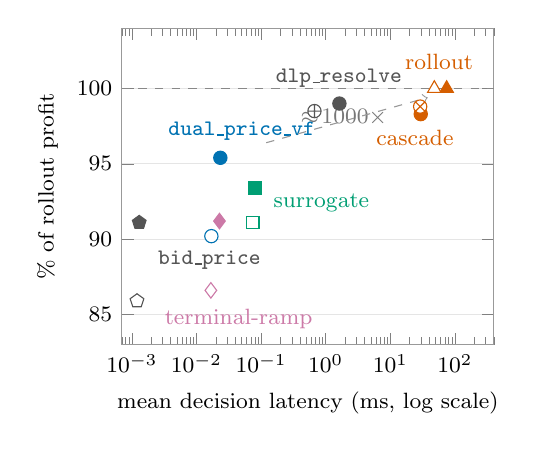
\begin{tikzpicture}
\begin{axis}[
  width=0.52\textwidth, height=5.6cm,
  xlabel={mean decision latency (ms, log scale)},
  ylabel={\% of rollout profit},
  xmode=log, xmin=0.0007, xmax=400,
  ymin=83, ymax=104,
  axis line style={mutedink!60},
  tick label style={font=\footnotesize},
  label style={font=\footnotesize},
  ymajorgrids, grid style={mutedink!15},
  clip=false,
]
\addplot[mutedink!70, dashed, thin, domain=0.0007:400] {100};
% tight = solid fill, scarce = open fill
\addplot[only marks, mark=pentagon*, mark size=2.6pt, mutedink]
  coordinates {(0.0013,91.1)};
\addplot[only marks, mark=pentagon*, mark size=2.6pt, mutedink, mark options={fill=white}]
  coordinates {(0.0012,85.9)};
\addplot[only marks, mark=diamond*, mark size=2.8pt, flatpink]
  coordinates {(0.0227,91.2)};
\addplot[only marks, mark=diamond*, mark size=2.8pt, flatpink, mark options={fill=white}]
  coordinates {(0.0167,86.6)};
\addplot[only marks, mark=*, mark size=2.4pt, vfblue]
  coordinates {(0.0234,95.4)};
\addplot[only marks, mark=*, mark size=2.4pt, vfblue, mark options={fill=white}]
  coordinates {(0.0170,90.2)};
\addplot[only marks, mark=square*, mark size=2.2pt, surteal]
  coordinates {(0.0807,93.4)};
\addplot[only marks, mark=square*, mark size=2.2pt, surteal, mark options={fill=white}]
  coordinates {(0.0748,91.1)};
\addplot[only marks, mark=triangle*, mark size=2.8pt, rollver]
  coordinates {(74.5,100)};
\addplot[only marks, mark=triangle*, mark size=2.8pt, rollver, mark options={fill=white}]
  coordinates {(48.0,100)};
\addplot[only marks, mark=oplus*, mark size=2.4pt, mutedink]
  coordinates {(1.63,99.0)};
\addplot[only marks, mark=oplus*, mark size=2.4pt, mutedink, mark options={fill=white}]
  coordinates {(0.67,98.5)};
\addplot[only marks, mark=otimes*, mark size=2.4pt, rollver]
  coordinates {(29.6,98.3)};
\addplot[only marks, mark=otimes*, mark size=2.4pt, rollver, mark options={fill=white}]
  coordinates {(29.0,98.8)};
\node[font=\footnotesize, mutedink, anchor=west] at (axis cs:0.0018,88.6) {\texttt{bid\_price}};
\node[font=\footnotesize, flatpink, anchor=north] at (axis cs:0.045,86.0) {terminal-ramp};
\node[font=\footnotesize, vfblue, anchor=south] at (axis cs:0.05,95.9) {\texttt{dual\_price\_vf}};
\node[font=\footnotesize, surteal, anchor=west] at (axis cs:0.11,92.4) {surrogate};
\node[font=\footnotesize, rollver, anchor=south] at (axis cs:57,100.6) {rollout};
\node[font=\footnotesize, mutedink, anchor=south] at (axis cs:1.6,99.4) {\texttt{dlp\_resolve}};
\node[font=\footnotesize, rollver, anchor=north] at (axis cs:24,97.9) {cascade};
\node[font=\footnotesize, mutedink!80, anchor=south] at (axis cs:1.9,96.9) {$\approx\!1000\times$};
\draw[mutedink!60, dashed, ->] (axis cs:0.12,96.4) -- (axis cs:38,99.4);
\end{axis}
\end{tikzpicture}%
\hfill
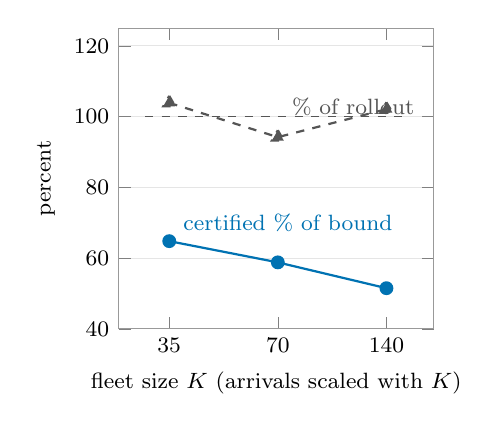
\begin{tikzpicture}
\begin{axis}[
  width=0.46\textwidth, height=5.4cm,
  xlabel={fleet size $K$ (arrivals scaled with $K$)},
  ylabel={percent},
  xtick={35,70,140}, xmode=log, log basis x=2,
  xticklabels={35,70,140},
  ymin=40, ymax=125,
  axis line style={mutedink!60},
  tick label style={font=\footnotesize},
  label style={font=\footnotesize},
  ymajorgrids, grid style={mutedink!15},
  clip=false,
]
\addplot[mutedink, dashed, thin, domain=30:160] {100};
\addplot[vfblue, thick, mark=*, mark size=2.1pt]
  coordinates {(35,64.8)(70,58.8)(140,51.5)};
\addplot[mutedink, thick, dashed, mark=triangle*, mark size=2.5pt]
  coordinates {(35,103.9)(70,94.2)(140,102.1)};
\node[font=\footnotesize, vfblue, anchor=west] at (axis cs:36,70) {certified \% of bound};
\node[font=\footnotesize, mutedink, anchor=south west] at (axis cs:72,97.5) {\% of rollout};
\end{axis}
\end{tikzpicture}
\caption{Left: the latency--quality frontier over thirty held-out seed
pairs (solid marks: tight; open marks: scarce). The log axis shows what
the tables cannot: \texttt{dual\_price\_vf} gives up 4.6--10 points of
rollout profit to move three orders of magnitude left; on tight it
sits above the rollout-trained surrogate at lower latency, on scarce
at the surrogate's level. Right:
proportional fleet scaling (cross-fitted, extension-matched
budgets). The policy tracks rollout (dashed, top)
while the certified fraction of the bound falls with $K$: the
reported gap widens with density under a common budget rule
(attribution between relaxation slack --- the mechanism
Theorem~\ref{thm:kernel} isolates --- residual dual
under-convergence, and
policy loss is open); the policy does not degrade against rollout.}
\label{fig:evidence}
\end{figure}

\begin{table}[t]
\centering
\caption{Proportional fleet scaling (tight economics), cross-fitted:
tables fitted from a different seed's solve of the same cell, the
policy and rollout simulated on the evaluation seed, and the bound
computed on that same evaluation seed --- a certificate requires the
bound and the realized policy value on the same instance, but the
tables can and should come from an independent stream (values
aggregated by evaluation stream, $\pm$ are sample standard
deviations, $n = 3$; driver script in the reproducibility appendix).
Bounds are extension-matched under a common rule: each cell's
size-scaled base solve plus one $+15$-iteration warm extension.
``Certified gap'' still means the \emph{reported} gap at those
budgets --- deeper convergence could narrow the levels --- so the
finding is the trend, not the levels.}
\label{tab:scaling}
\small
\begin{tabular}{rrr}
\toprule
$K$ & certified gap & policy vs rollout \\
\midrule
35 & 35.2 $\pm$ 1.3\% & 103.9 $\pm$ 4.1\% \\
70 & 41.2 $\pm$ 1.6\% & 94.2 $\pm$ 2.0\% \\
140 & 48.5 $\pm$ 1.8\% & 102.1 $\pm$ 2.6\% \\
\bottomrule
\end{tabular}
\end{table}

The certificate gap widens with density under extension-matched
budgets (Table~\ref{tab:scaling}: each cell's size-scaled base solve
warm-extended one $+15$-iteration round under a common rule,
$35.2 \to 41.2 \to 48.5\%$), and the widening replicates across
seeds with tight dispersion. The extensions still improved most
incumbents at their final iterations, so deeper convergence could
narrow the levels further: we read the trend, not the levels, as the
finding, and the cross-$K$ comparison still partially confounds
density with residual dual convergence. Cross-fitting
(\path{scripts/run_scaling_crossfit.sh}) turns out to
be immaterial here --- the in-sample fresh-seed values differ from
the cross-fitted ones by at most $0.1$~pp --- but the table reports
the cross-fitted design because only it is deployment-valid. The
policy stays within 7\% of
rollout at all scales, beating it at $K = 35$ and at
$K = 140$. None of this separates
relaxation slack from policy loss; for that attribution, see the exact
micro study below. Rollout's latency
grows $32 \to 159$\,ms over this
range; the dual policy stays ${\sim}0.1$\,ms.

\paragraph{Portability and solver budgets.} On the tested pairs,
outcomes are identical in aggregate (equal profits and accept counts;
we did not compare full decision sequences) under frozen (pair-0) vs
freshly solved (pair-1) duals on both stress scenarios
--- consistent with Lemma~\ref{lem:stability}'s basis stability.
Bound-grade certificates require ${\sim}45$ subgradient iterations;
the headline tables were fitted from 15--50-iteration solves, and we
have not established a minimal policy-grade budget (no
decision-invariance comparison across budgets is included in the
artifacts). Per-resource solves parallelize at $3.05\times$ on four
cores.

\FloatBarrier
\paragraph{Exact attribution at micro scale.} The certificate-gap
attribution question is answerable exactly where the joint optimum is
computable. On micro instances we compute four quantities on one
objective (\path{scripts/run_joint_optimum.py}): the exact
chain-packing LP value ($= \min_{\lambda} L$, rational simplex), the
exact \emph{joint} accept-and-assign optimum $\Vstar$ (memoized
exhaustive search; unlike the benchmark's hindsight DP it fixes
neither the accept nor the dispatch rule), the exact best accept
sequence under the benchmark's fixed dispatch rule, and the simulated
policy. The \emph{primary design} guards against hindsight-adaptive
construction: each instance draws a random 24-hour window over the
horizon, thins the window's loads to $L = 20$ so arrivals span it
(service chains of length 3--4 become feasible, and every instance
realizes a chain of length $\geq 3$), restricts to the top-six FAF
origin markets by an ex-ante rule of the lane data, and places $K = 3$
trucks by the benchmark's own FAF-weighted draw --- never observing
the realized loads. Across thirty such instances (tight and scarce,
fifteen each), the exact rational simplex --- run over rewards and
terminal values quantized to integer cents before every computation,
so ``exact'' means exact over the monetary inputs, not over
rationalized binary floats --- finds an \emph{integral}
optimal solution (a feasible joint assignment, so
$\min_{\lambda} L = \Vstar$ combinatorially; finding one integral
optimum does not make the polytope integral) on 26 of 30; pooled over all instances the
certificate gap decomposes as $0.3\%$ relaxation slack, $12.0\%$
dispatch-rule cost, and $87.7\%$ policy accept loss. Dispatch cost is
heterogeneous across instances (per-instance share: median $8.3\%$,
mean $17.2\%$, max $89\%$, exactly zero on 9/30), so we report the
distribution rather than the pooled share alone. The earlier
stream-prefix design (thirty instances, $K = 4$--$5$ trucks placed on
the prefix's busiest markets --- a hindsight-adaptive initial
condition with chains of length $\leq 2$) is retained for comparison:
there the LP is integral on 30/30 and dispatch cost pools to $14.6\%$
(per-instance median $2.9\%$, zero on 12/30). At micro scale, under
both designs, the certified gap is overwhelmingly money left by the
\emph{policy}, not by the bound; whether that attribution persists at
benchmark scale, where kernel-like contention structures have more
room to arise, remains open.

\paragraph{Portability across training realizations.} Basis
stability (Remark~\ref{rem:portability}) predicts fitted prices are
interchangeable across sample paths. In the \emph{tight} scenario
(the only one tested), we fit tables from five
independent 72-hour training realizations (the canonical stream plus
four independent certificate-program streams) and evaluate each on the
same twenty held-out pairs. Every arm's mean retention lands within
$0.07$~pp of the canonical arm's $95.3\%$; on any given evaluation
stream, swapping the training realization moves retention by
$0.10$~pp on average and never more than $0.71$~pp. One solve prices
many operating horizons --- across $5 \times 20$
training--evaluation cells, not a single comparison. This is
consistent with the basis-stability mechanism, though the benchmark
generator violates several of Theorem~\ref{thm:fluid}'s assumptions,
so it is consistency, not confirmation.

\paragraph{A low-contention family: the theorem-inspired policy, out
of sample.} Theorem~\ref{thm:fluid}
and Corollary~\ref{cor:tight} cover a lane-priced, soft-margin policy
under (A1)--(A4). We built that policy
(\path{scripts/fit_dual_prices.py} with \texttt{--granularity lane};
acceptance margin \$50) and a low-contention scaling family (mild
economics, fleet/demand
ratio raised to 10; cells at $K = 60/120/240$, three seed pairs each),
and evaluated it \emph{out of sample}: for every ordered pair of
seeds, tables fitted from one seed's dual solve are scored on the
other seed's stream (\path{scripts/run_subcritical_crossfit.py}) ---
the independence the theorem requires. Aggregated by evaluation
stream (three independent streams, each scored under two independent
training tables), cross-fitted certified fractions are numerically
close to the in-sample results
($64.3 \pm 1.1$, $59.3 \pm 3.0$, $45.5 \pm 1.1\%$ at the deepest
solver budgets), and mean retention vs rollout is $110.4$, $104.5$,
and $100.2\%$ (three evaluation streams per cell; at $K = 240$ one
stream's mean falls below rollout) --- consistent with basis
stability.

Two caveats scope what this tests. First, instrumented diagnostics
show the family is \emph{not} (A1)-subcritical: idle pools do empty,
and 20--26\% of arrivals are blocked by the feasibility guard despite
otherwise-accepting scores. FAF-calibrated geography has structurally
thin markets, so ``idle mass in every market'' fails at any aggregate
fleet ratio. Second, the scenario retains the benchmark's windows,
HOS clocks, stochastic yard delays, and heterogeneous rewards, which
(A2)--(A4) idealize away. This experiment is therefore a
low-contention, out-of-sample robustness test of the
theorem-\emph{inspired} policy, not a validation of the theorem's
hypotheses; the assumption-matched family below tests those
directly.

The certificate side of this iteratively solved low-contention
family ($K = 60/120/240$, subgradient budgets) stands on its own. At
the 25-iteration base budget the certified fractions read
$57.6/49.2/41.4\%$; warm-extending the same solves to 70 iterations
lifts them to $64.4/59.0/45.6\%$ --- with dual trajectories still
descending.
Reported
certificates climb monotonically with solver effort --- the direction
the conservativeness remark after Corollary~\ref{cor:tight}
predicts. Any cross-$K$ comparison at a
\emph{fixed} iteration budget confounds scale with dual convergence,
since larger instances are further from their optimal duals at the
same budget. The corollary's large-$K$ tightening is therefore not
testable at these budgets: the experiment is consistent with, but
does not confirm, asymptotic certificate tightness.

\paragraph{Theorem 2 on its own terms.} Because the benchmark
violates (A1)--(A4), we also built the idealized model the theorem
actually analyzes and ran the paper's own pipeline on it
(\path{scripts/run_matched_family.py}): four markets on a directed
cycle; independent Poisson cell counts arriving at integer hour
epochs; integer occupation time; zero within-cell reward dispersion;
\emph{nonconstant} terminal values ($V = 500/400$ alternating), so
fluid thresholds are $\pm\$100$, lane rents differ by lane
($\$700$/$\$900$), and the spatial gradient is materially nonzero;
profitable forward and unprofitable reverse lanes; $50\%$
utilization (A1); no windows, clocks, or delays (A2 exact). Each of
thirty train/evaluation pairs per fleet size solves the training
realization's relaxation to numerical optimality --- the cell-level
arc-flow LP of Lemma~\ref{lem:stability}(c) under the repository's
float simplex, whose demand-row duals are the
optimal sample-path prices the theorem stipulates (the benchmark uses
a subgradient solver because its trucks are heterogeneous; this
family's exact interchangeability degenerates the subgradient and
makes the LP the right solver) --- fits the lane--hour table with the
production fitter's five-pseudo-observation shrinkage rule and the
$\widehat{W}$ recursion from that solve, and scores the
independently solved evaluation path. Both convergence statements
hold as predicted across $K = 48$ to $768$ ($\pm$ values are sample
standard deviations over the thirty pairs): the certified fraction
rises $70.2 \pm 14.8 \to 82.3 \to 91.7 \to 97.7 \to
99.8 \pm 1.3\%$ and the per-truck gap falls
$\$819 \to \$502 \to \$235 \to \$65 \to \$6.6$. Without
shrinkage --- the theory-aligned sensitivity variant, since the
theorem assumes per-cell fits --- the same curve reads
$84.5 \pm 6.6 \to 99.9 \pm 0.6\%$
(\path{benchmark_runs/trackb/matched_family_unshrunk.csv}):
shrinkage biases small-$K$ prices toward lane means and slows the
approach without changing the limit. The
diagnostics track the theory's internal quantities: fitted-price RMSE
against the known fluid rents falls $\$147 \to \$5$
(Lemma~\ref{lem:stability}), the maximum $\widehat{W}$ error
against the pinned $\omega V$ falls $\$517 \to \$10$
(Lemma~\ref{lem:wcons}), and the fraction of evaluation paths with
zero guard blocks rises from $0/30$ to $29/30$ --- blocking becomes
rare but is not guaranteed absent at any finite $K$. This validates
the theorem's mechanism on its own model; the distance between this
family and FAF-calibrated geography is precisely the content of the
caveats above.

\section{Discussion}
\label{sec:discussion}

\paragraph{A certificate culture for freight decisioning.} Every policy
run on the benchmark can now report ``provably $\geq x\%$ of the
hindsight optimum on this instance'' (the additive bound of
Theorem~\ref{thm:cert} is unconditional; the \emph{fraction} is
meaningful when the policy value and bound are positive, as they are
in every run here). The certifier is policy-agnostic --- Table~\ref{tab:certs}
certifies the rollout teacher and the re-solving DLP with the same
bound --- and \S\ref{sec:limits} shows why certificates can be
irreducibly conservative on some instance families (whether the
benchmark's instances contain that mechanism remains open). The observable decomposition ---
policy value, rollout value, bound --- separates what stronger
policies of the tested classes have achieved from what remains as
certificate gap; the exact micro study splits that remainder where the
joint optimum is computable (relaxation slack $0$--$0.3\%$ pooled
across the two designs; the gap is policy loss), and benchmark-scale
attribution remains open.

\paragraph{Relation to the benchmark's cascade.} On the same thirty
pairs (Table~\ref{tab:headline}), the v0.3 surrogate-to-rollout
cascade \citep{chandrasekaran2026freightbidbench} attains
$98.3$--$99.5\%$ of rollout. But it needs 200
rollout labels per stream to train, and it invokes rollout on
escalated decisions (18--30\,ms mean latency). On the stress
scenarios the dual policy trades 3--9 retention points for
${\sim}500\times$ lower latency and no teacher labels (on mild it
beats the cascade outright).
The two are complementary. Replacing the cascade's cheap stage with the
dual policy is a natural follow-up, and we leave it to future work.

\paragraph{Prices are infrastructure.} Basis stability makes the fitted
price surface a reusable asset: each of five training solves was
reused unchanged across twenty evaluation streams (tight scenario)
with at most a $0.71$~pp effect. There is a testable warning condition --- arrival-regime
switches --- for when to refit. Per-request-learning schemes do not
offer this property.

\paragraph{Where the money is.} The exact micro study points the
finger at the policy, not the bound: where the joint optimum is
computable, relaxation slack is negligible in aggregate ($0.3\%$ of
the certificate gap in the primary design, zero in the legacy design)
and the gap is accept loss plus dispatch cost. If that attribution persists at scale, the
next methodological target is stronger accept rules (quantile prices
for heterogeneous rewards, Remark~\ref{rem:heterogeneous}; smarter
dispatch) rather than tighter bounds. If instead kernel-like
contention emerges at scale --- \S\ref{sec:limits} shows it can ---
bound-tightening via chain-aware duals or restricted exchange
constraints becomes the lever, with Theorem~\ref{thm:kernel}'s kernel
families as test cases. The low-contention convergence experiment adds
the third ingredient: certificate tightness at scale is also a
\emph{compute} question, since reported gaps shrink monotonically with
solver iterations.

\section{Limitations}
\label{sec:limitations}

Certificates inherit the bound's looseness. In the critical regime they
understate policy quality (Table~\ref{tab:certs}'s rollout column), and
Theorem~\ref{thm:fluid} does not apply there; the critical case is
open. Assumption (A2) folds HOS-clock renewal into the regime
definition, and relaxing it needs a regeneration argument. The
surrogate baseline is the benchmark's dependency-free linear model, not
a tuned learned policy; rollout is the strong baseline. All evidence
is synthetic: the benchmark is calibrated to public data, and there
has been \emph{no validation against real carrier operations} ---
no operational deployment, no comparison to carrier decision logs.
Benchmark caveats --- lane concentration among them --- carry over
from the v0.3 release \citep{chandrasekaran2026freightbidbench}. We defer
the online-updating variant and a learned deferral rule to future work,
by scope discipline.

\section{Conclusion}
\label{sec:conclusion}

One Lagrangian relaxation plays two separate roles: fitted once, it
yields a microsecond, rollout-label-free, portable acceptance policy;
computed ex post on a realized stream, it certifies any policy's
optimality gap on that instance. The theory says when the
certificate is tight (subcritical fluid consistency,
Theorem~\ref{thm:fluid} with Corollary~\ref{cor:tight}) and shows,
with exact certificates, why it cannot always be (kernels with
irreducible per-resource slack, Theorem~\ref{thm:kernel}). On a public
benchmark the policy beats a rollout-trained surrogate on two of three
scenarios (no statistically detectable difference on the third), at
roughly three orders of magnitude lower
latency than the teacher; a cadence-tuned re-solving deterministic LP
--- the strongest zero-label baseline once its duration conventions
match the simulator's --- out-earns the static policy on the two
stress scenarios, and the same ex-post certifier prices it on the
same scale. The contribution is the characterized static policy and
the certificate practice, not profit dominance over re-solving. We
release the benchmark, the solver, the
kernel search, and every table for independent verification.

\section*{Declaration of Competing Interest}

The author is employed by Bubba AI, which develops AI-based
load-planning and carrier-operations products in the freight domain
addressed by this paper. This study uses only public data and the
open-source benchmark; no proprietary data or systems were used, and
Bubba AI had no role in the study design, the analysis, or the decision
to publish.

\section*{Acknowledgements}

The author used Anthropic's Claude, a large language model, to assist
with software implementation and experiment scaffolding, drafting and
editing of the manuscript, and literature and formatting support. All
model designs, proofs, experiments, results, and claims were verified
and approved by the author, who takes full responsibility for the
content.

\appendix

\section{Completing the Proof of Theorem~\ref{thm:fluid}: the
Fleet-Coupling Estimate}
\label{sec:coupling}

This appendix proves Step~4 of Theorem~\ref{thm:fluid} in full. The
argument is simpler than the mean-field coupling one might expect, for
one structural reason: \emph{under the (A2)--(A4) idealization, the
policy analyzed here is state-blind}. In the hourly model, feasible
idle resources are homogeneous --- rest-inclusive occupation times
renew clocks (A2) and rewards are cell-homogeneous (A4) --- so the
score of the idealized policy depends only on the load's features and
the clock, never on which resource serves, except through the
feasibility guard, which requires one idle resource at the origin.
(The \emph{deployed} policy is not literally state-blind: it scores
the selected truck's realized profit and actual schedule completion,
which depend on fleet and HOS state; under (A2)--(A4) those
distinctions vanish and the two coincide.) So, as long as
no market's idle pool is exhausted, the dispatch process is a
deterministic thinning of the arrival stream, and there is no feedback
loop between fleet state and decisions to control. The proof therefore
has three parts: a uniform concentration bound on arrivals
(Lemma~\ref{lem:conc}), an agreement lemma matching policy decisions to
fluid decisions (Lemma~\ref{lem:agree}), and an epoch induction with
whole-batch concentration
showing the idle pools never empty (Lemma~\ref{lem:track}). A value
ledger (Proposition~\ref{prop:ledger}) then completes Steps 4--5 of the
theorem.

\subsection{The soft acceptance margin}
\label{sec:margin}

One honest repair to the policy is needed first. Under within-cell
homogeneity (A4), a fluid-\emph{served} cell has fitted rent
$\hat{\lambda} \approx \bar{r} - \theta$ and gradient
$g \approx -\theta$, so the score of a served load is
\begin{equation}
  \mathrm{score} \;=\; r - \hat{\lambda} + g
  \;\approx\; \bar{r} - (\bar{r} - \theta) - \theta \;=\; 0.
\end{equation}
Served cells sit \emph{exactly at the acceptance boundary}: the rent
cancels the surplus. This knife edge is not an artifact of our policy;
it is the classical degeneracy of bid-price controls at the fluid
optimum \citep{talluri1998bidprice}, usually repaired by booking limits
or perturbed prices. We repair it with a soft margin.

First extend the nondegeneracy assumption with an explicit
threshold-separation constant.

\begin{assumption}[A3$'$: threshold separation]
\label{ass:sep}
No cell sits at its threshold:
\begin{equation}
  \eta \;:=\; \min \bigl\{\, \theta_{\ell h} - \bar{r}_{\ell}(h)
  \;:\; \text{cell } (\ell, h) \text{ fluid-rejected} \,\bigr\}
  \;>\; 0,
  \label{eq:margin}
\end{equation}
and every fluid-served cell is served in full
($u_{\ell} = \Lambda_{\ell}$ on the cell).
\end{assumption}

(A3$'$) adds to (A3) --- which already assumes a unique,
nondegenerate global optimal basis --- two cellwise conditions:
threshold separation and full-or-zero service. A cell with
$\bar{r} = \theta$ admits a continuum of alternative primal optima,
which (A3$'$) excludes. Under (A4) the dual data are constant on each
hourly cell (and the epoch LP has one global optimal basis), so
\eqref{eq:margin} is a minimum over finitely many well-defined cells.

Two conventions used throughout the appendix. \emph{Durations:}
$\tau_{\ell}$ is the deterministic, rest-inclusive occupation time of
\S\ref{sec:fluid}: a resource dispatched at $t$ is occupied on
$[t, t + \tau_{\ell})$ and is idle in market $\delta_{\ell}$ from
$t + \tau_{\ell}$ with renewed clocks, hence feasible for any
subsequent in-market arrival by (A2). A resource still resting at $T$
is physically at its destination, so the model's terminal value
$\Phi$ credits $V(\delta_{\ell})$ --- consistent with the pipeline
term $\tilde{z}$ in \eqref{eq:fluid}. Stochastic duration noise
(yard delays) would move completions off the epoch grid --- the same
off-grid aggregation gap Remark~\ref{rem:gridgap} leaves open --- so
it is excluded by (A4), not handled here. \emph{Tables:} $\hat{\lambda}$ and $\widehat{W}$ are hourly.
Under the grid-alignment clause of (A4) every completion time
$t + \tau_{\ell}$ lies on the grid and advances it by at least one
cell ($\tau_{\ell} \geq 1$); the deployed implementation, whose
event-time completions are off-grid, reads the value of the containing
hour.

Let $\delta_K$ denote the within-cell reward dispersion of (A4) plus
the table-fit error of Lemma~\ref{lem:stability}, so
$\delta_K \to 0$. Fix any sequence $\varepsilon_K$ with
\begin{equation}
  3\,\delta_K \;\leq\; \varepsilon_K \;\leq\; \eta / 2,
  \label{eq:margincond}
\end{equation}
which exists for $K$ large since $\delta_K \to 0$. The
\emph{$\varepsilon$-margin policy} $\pol^{\varepsilon}$ accepts iff
$\mathrm{score} \geq -\varepsilon_K$ (and a feasible resource exists);
Theorem~\ref{thm:fluid} is stated for $\pol^{\varepsilon}$.

\begin{remark}
The benchmark policy uses $\varepsilon = 0$. In practice rewards within
a cell are genuinely heterogeneous, contested cells have interior
thresholds, and the zero-margin rule is not degenerate
(Remark~\ref{rem:heterogeneous}); the margin is a proof device for the
homogenized limit, not a change to the deployed policy. Its width
depends on the unobservable constants $\eta$ and $\delta_K$ --- it is
an existence statement, not a tuning recipe.
\end{remark}

\begin{remark}[Table granularity]
\label{rem:granularity}
The theorem analyzes tables fitted at \emph{lane--hour} granularity
(origin, destination, hour), matching the cell structure of the fluid
LP: the rent $\lambda_{\ell}(h) = (\bar{r}_{\ell}(h) -
\theta_{\ell h})_+$ depends on the destination through
$\theta_{\ell h}$, so two lanes sharing an origin generically carry
different rents. The deployed table of \S\ref{sec:surrogates} pools
by \emph{market--hour} (with shrinkage), i.e., it stores a
demand-weighted mixture of lane rents. The two coincide exactly when
rents are homogeneous within each origin--hour; otherwise the pooled
table over-shades served lanes whose rent is below their origin's
average, by exactly the within-origin rent dispersion. The pooled
variant trades this bias for lower estimation variance --- the
empirical choice of \S\ref{sec:experiments} --- but the guarantee of
Theorem~\ref{thm:fluid} is proved for the lane-granular variant.
\end{remark}

\subsection{Uniform concentration of arrivals}

Work in the discrete-epoch model of (A4): the cell counts
$N_{\ell h}$ are independent Poissons with means
$K \mu_{\ell h} = K \int_h^{h+1} \Lambda_{\ell}(s)\, ds$, and all
events happen at the $T + 1$ hour epochs, so suprema over continuous
time reduce to maxima over epochs. Write
$N_{\ell}(h) = \sum_{h' < h} N_{\ell h'}$ for the epoch partial
sums, $\mu_{\ell}(h)$ for their means, and
$\Lambda_{\max} := \max_{\ell} \sup_{t} \Lambda_{\ell}(t)$.

\begin{lemma}[Uniform arrival concentration]
\label{lem:conc}
Let $E_1$ be the event
\begin{equation}
  \max_{\ell \in L}\; \max_{h \leq T}\;
  \bigl| N_{\ell}(h) - K \mu_{\ell}(h) \bigr|
  \;\leq\; a_K \;:=\; \sqrt{6\, \Lambda_{\max} T\, K \log K}.
\end{equation}
Then $\Pr(E_1) \geq 1 - O(K^{-2})$.
\end{lemma}

\begin{proof}
\emph{Step 1.} Each partial sum $N_{\ell}(h)$ is Poisson with mean
$K \mu_{\ell}(h) \leq K \Lambda_{\max} T$.

\emph{Step 2.} The Poisson Bernstein bound gives, for each lane and
epoch,
$\Pr\bigl( |N_{\ell}(h) - K\mu_{\ell}(h)| \geq a \bigr)
\leq 2 \exp\bigl( -a^2 / (2 K \Lambda_{\max} T + 2a/3) \bigr)$
(equivalently, Freedman's inequality \citep{freedman1975tail} for the
discrete-time martingale of partial sums).

\emph{Step 3.} Take $a = a_K$: the exponent is at most
$-3 \log K + o(\log K)$ for $K$ large. A union bound over the
$|L| (T + 1)$ lane--epoch pairs --- a constant independent of $K$ ---
gives $\Pr(E_1^c) = O(K^{-2})$.
\end{proof}

\subsection{The value-to-go table is consistent}

\begin{lemma}[$\widehat{W}$-consistency]
\label{lem:wcons}
Under (A1)--(A4), on the basis-stability event of
Lemma~\ref{lem:stability} (training path, optimal duals), the backward
recursion \eqref{eq:wrec} satisfies, for a constant $C$ depending only
on $T$,
\begin{equation}
  \max_{m, t}\; \bigl| \widehat{W}(m, t) - \omega V(m) \bigr|
  \;\leq\; C\,\delta_K,
  \qquad\text{hence}\qquad
  \bigl| g(\ell, h) + \theta_{\ell h} \bigr| \;\leq\; 2 C\,\delta_K
  \;\;\text{for every cell.}
\end{equation}
\end{lemma}

\begin{proof}
Let $\epsilon(t) = \max_m |\widehat{W}(m, t) - \omega V(m)|$ on the
hourly grid.

\emph{Step 1 (base).} $\widehat{W}(m, T) = \omega V(m)$ by definition,
so $\epsilon(T) = 0$.

\emph{Step 2 (wait branch).} The wait branch of \eqref{eq:wrec}
contributes $\widehat{W}(m, t{+}1) \geq \omega V(m) - \epsilon(t{+}1)$,
so $\widehat{W}(m, t) \geq \omega V(m) - \epsilon(t{+}1)$: the
recursion never falls more than the next step's error below the pin.

\emph{Step 3 (dispatch branches).} A dispatch branch contributes
$r_i - \lambda_i + \widehat{W}(\delta, t + \tau_{\ell})$. On the
stability event the training dual of load $i$ is
$\lambda_i = (r_i - \hat{\theta}_{\ell h})_+$
(Lemma~\ref{lem:stability}, Step~2), so
$r_i - \lambda_i = \min(r_i, \hat{\theta}_{\ell h}) \leq
\theta_{\ell h} + \delta_K$. Since
$\theta_{\ell h} = \omega [V(o_{\ell}) - V(\delta_{\ell})]$ under the
pinning of Lemma~\ref{lem:flat}, the branch is at most
$\omega V(o_{\ell}) + \delta_K + \epsilon(t + \tau_{\ell})$.

\emph{Step 4 (recursion).} Every dispatch branch lands strictly later
on the grid --- $\tau_{\ell} \geq 1$ by the grid-alignment clause of
(A4), so $t + \tau_{\ell} \geq t + 1$ and the induction is
well-founded. Combining,
$\epsilon(t) \leq \max_{s > t} \epsilon(s) + 2 \delta_K$, and backward
induction over the at most $T$ grid steps gives
$\epsilon(t) \leq 2 T \delta_K$. The gradient statement follows from
$g(\ell, h) = \widehat{W}(\delta, \cdot) - \widehat{W}(o, \cdot)$ and
the triangle inequality.
\end{proof}

\subsection{Decisions agree with the fluid}

Let $E_2$ be the basis-stability event of
Lemma~\ref{lem:stability} for the (independent) training path: on
$E_2$ the frozen tables satisfy
$|\hat{\lambda}(\ell, h) - \lambda_{\ell}(h)| \leq \delta_K$
(Lemma~\ref{lem:stability}(b)) and
$|g(\ell, h) + \theta_{\ell h}| \leq \delta_K$
(Lemma~\ref{lem:wcons}, absorbing its constant into $\delta_K$) for
every cell, and $\Pr(E_2) = 1 - o(1)$. Note $E_2$ is a single event
about the frozen tables --- it is not re-drawn per decision. By the
hour-grid clause of (A4), every cell lies strictly inside one dual
regime: the dual data are constant on every cell.

\begin{lemma}[Decision agreement]
\label{lem:agree}
On $E_2$, for every arrival whose origin market has
an idle feasible resource: $\pol^{\varepsilon}$ accepts iff the cell is
fluid-served.
\end{lemma}

\begin{proof}
\emph{Step 1 (served cells).} Let the cell be fluid-served, so
$\bar{r} \geq \theta$ and $\lambda_{\ell}(h) = \bar{r} - \theta$. The
load's reward is $r = \bar{r} \pm \delta_K$ by (A4). Then
\begin{equation}
  \mathrm{score}
  = r - \hat{\lambda} + g
  \;\geq\; (\bar{r} - \delta_K) - (\bar{r} - \theta + \delta_K)
  - (\theta + \delta_K)
  \;=\; -3\,\delta_K
  \;\geq\; -\varepsilon_K,
\end{equation}
using \eqref{eq:margincond}. The policy accepts.

\emph{Step 2 (rejected cells).} Let the cell be fluid-rejected, so
$\bar{r} \leq \theta - \eta$ by \eqref{eq:margin} and
$\lambda_{\ell}(h) = 0$, hence $\hat{\lambda} \geq 0$ always. Then
\begin{equation}
  \mathrm{score}
  \;\leq\; (\bar{r} + \delta_K) - 0 - (\theta - \delta_K)
  \;\leq\; -\eta + 2\,\delta_K
  \;<\; -\varepsilon_K,
\end{equation}
since $\varepsilon_K \leq \eta/2$ and $2\delta_K < \eta/2$ for $K$
large. The policy rejects.
\end{proof}

\subsection{Occupancy tracks the fluid; no forced rejections}

Let $X^{-}_m(h)$ be the number of idle resources in market $m$ at
epoch $h$ after completions release and before the batch is processed
(Remark~\ref{rem:hourlyreading}), and $X^{+}_m(h)$ the count after
the batch; deterministic proportional initial placement gives
$X^{-}_m(0) = K z^0_m + O(1)$ (rounding only). Let $S_{\ell}(h)$
count dispatches on lane $\ell$ in batches $0, \dots, h$. Define the
deviation
\begin{equation}
  D(h) \;=\; \sum_{m} \bigl| X^{-}_m(h) - K z^{-}_m(h) \bigr|,
\end{equation}
comparing pre-batch stochastic inventory with the pre-batch fluid
inventory $z^{-}_m(h)$ of \eqref{eq:epochlp} (at $h = H$ there are
no dispatches, so $z^{-}_m(H) = z_m(H)$).

\begin{lemma}[Occupancy tracking]
\label{lem:track}
On $E_1 \cap E_2$, for all $K$ large:
$\max_{h \leq T} D(h) \leq C \sqrt{K \log K}$, and at every epoch
and every position within every batch the arrival's origin pool is
nonempty. In particular no accepted arrival is ever rejected
for lack of an idle resource, and under (A2) every accepted arrival is
served.
\end{lemma}

\begin{proof}
By induction over epochs. The induction hypothesis $H(h)$: in every
batch before epoch $h$, exactly the fluid-served cells' arrivals were
dispatched (none was blocked), and the epoch deviations satisfy the
stated bound up to $h$.

\emph{Step 1 (flow identity).} Idle counts change only by dispatches
out and service completions in:
\begin{equation}
  X^{-}_m(h) = X^{-}_m(0)
  + \sum_{\ell:\, \delta_{\ell} = m} S_{\ell}(h - \tau_{\ell})
  - \sum_{\ell:\, o_{\ell} = m} S_{\ell}(h - 1),
\end{equation}
with $S_{\ell}$ vanishing at negative indices.
The pre-batch fluid mass $z^{-}_m(h)$ satisfies the same
cumulative identity with $K \sum u_{\ell}$ in place of $S_{\ell}$
(unrolling the balance rows of \eqref{eq:epochlp}).

\emph{Step 2 (dispatches are thinned arrivals under $H(h)$).} Under
$H(h)$, the dispatch counts entering Step~1's identity at epoch $h$
are exactly the arrival counts of fluid-served cells: the accept set
is a deterministic union of cells given the frozen tables ---
acceptance is all-or-nothing per cell under (A4) homogeneity
(Lemma~\ref{lem:agree}) --- and no arrival in those cells was
blocked. This thinning is adapted (no decision peeks at the future),
and the fluid serves the full arrival mass of served cells
(Assumption~\ref{ass:sep}), so Lemma~\ref{lem:conc} gives
\begin{equation}
  \max_{h' < h}\,
  \bigl| S_{\ell}(h') - K \textstyle\sum_{h'' \leq h'} u_{\ell}(h'') \bigr|
  \;\leq\; C_1\, a_K
\end{equation}
--- strictly before the current batch, which $H(h)$ covers; once
Step~4 certifies batch $h$, the same bound extends through $h$ and
feeds the next induction step. Step~1's identity at epoch $h$ only
consumes dispatch counts at indices $\leq h - 1$
($\tau_{\ell} \geq 1$), so this suffices; the constant $C_1$ absorbs
the conversion from initial-segment deviations to the finitely many
served-cell intervals.

\emph{Step 3 (deviation bound at epoch $h$).} Plug Step~2 into
Step~1: $X^{-}_m(h) - K z^{-}_m(h)$ is a signed sum of at most $2|L|$
dispatch deviations plus the $O(1)$ initial rounding error, so
\begin{equation}
  D(h) \;\leq\; 2 |M| \, |L| \, C_1\, a_K + O(1)
  \;=\; O\bigl( \sqrt{K \log K} \bigr).
\end{equation}

\emph{Step 4 (the whole batch at epoch $h$ is safe).} Within batch
$h$, pools only decrease, and the total decrement at market $m$ ---
no matter which prefix of the batch has been processed --- is at most
the batch's fluid-served arrival count at $m$. A single batch count
is a difference of two cumulative counts, so its deviation is at most
$2 a_K$ per lane on $E_1$; summing over $m$'s outbound lanes, the
decrement is at most
$K \sum_{\ell: o_{\ell} = m} u_{\ell}(h) + C_2 a_K$ with
$C_2 = 2|L|$ (rejected cells never decrement a pool: their scores
reject regardless of pool state). Hence every within-batch prefix
inventory is at least
\begin{equation}
  X^{-}_m(h) - K \textstyle\sum_{\ell: o_{\ell} = m} u_{\ell}(h)
  - C_2 a_K
  \;\geq\; K z_m(h) - D(h) - C_2 a_K
  \;\geq\; z_{\min} K - O(\sqrt{K \log K})
  \;>\; 0
\end{equation}
for $K$ large --- the first inequality uses
$X^{-}_m(h) \geq K z^{-}_m(h) - D(h)$ and
$z^{-}_m(h) - \sum_{\ell: o_{\ell}=m} u_{\ell}(h) = z_m(h)$, the
second the post-batch clause of (A1). No pool empties at
any position inside batch $h$, so no arrival is blocked, every
fluid-served arrival is dispatched, and $H(h{+}1)$ holds. The
induction needs no first-violation device: the prefix bound is
uniform over the batch because the worst-case decrement is the whole
batch's served mass, independent of which loads have been processed.
\end{proof}

\subsection{The value ledger}

\begin{proposition}[Steps 4--5 of Theorem~\ref{thm:fluid}]
\label{prop:ledger}
Under (A1)--(A4), (A3$'$), and \eqref{eq:margincond},
$V^{\pol^{\varepsilon}}(K) \geq V_f K - o(K)$.
\end{proposition}

\begin{proof}
\emph{Step 1 (restrict to the good event).} Rewards may be negative,
so we truncate rather than discard. Pathwise,
$|\text{value}| \leq r_{\max} N + \omega V_{\max} K$ with $N$ the
total arrival count. Against $E_1^c$: Cauchy--Schwarz with
$\mathbb{E}[\text{value}^2] = O(K^2)$ (Poisson second moment) and
$\Pr(E_1^c) = O(K^{-2})$ (Lemma~\ref{lem:conc}) gives
$\mathbb{E}[|\text{value}|\,\mathbf{1}_{E_1^c}]
\leq (\mathbb{E}\,\text{value}^2)^{1/2} \Pr(E_1^c)^{1/2}
= O(K) \cdot O(K^{-1}) = o(K)$. Against $E_2^c$: the realized value depends on the training path
through the tables, but its envelope
$r_{\max} N + \omega V_{\max} K$ depends only on the evaluation
path and is independent of $E_2$, so
$\mathbb{E}[|\text{value}|\,\mathbf{1}_{E_2^c}]
\leq (r_{\max} \mathbb{E}[N] + \omega V_{\max} K) \Pr(E_2^c)
= O(K) \cdot o(1) = o(K)$. Hence
$V^{\pol^{\varepsilon}}(K) \geq
\mathbb{E}\bigl[ \text{value} \cdot \mathbf{1}_{E_1 \cap E_2} \bigr]
- o(K)$.

\emph{Step 2 (dispatch reward).} On the good event, by
Lemmas~\ref{lem:agree}--\ref{lem:track} the served set matches the
fluid-served set up to counting fluctuations of
$O(\sqrt{K \log K})$ per lane. With rewards bounded by $r_{\max}$ and
within-cell dispersion $\delta_K$,
\begin{equation}
  \sum_{\text{served}} r
  \;\geq\; K \sum_{h < H} \sum_{\ell} \bar{r}_{\ell}(h)\, u_{\ell}(h)
  \;-\; r_{\max}\, O(\sqrt{K \log K})
  \;-\; \delta_K\, O(K).
\end{equation}

\emph{Step 3 (terminal value).} The realized terminal value credits
idle resources at their market and in-transit resources at their
destination, matching the epoch LP's terminal terms in
\eqref{eq:epochlp}. The idle part
deviates from $\omega \sum_m V(m) K z_m(H)$ by at most
$\omega V_{\max} D(H)$; the in-transit part per lane is
$S_{\ell}(H{-}1) - S_{\ell}(H - \tau_{\ell})$ (batches end at
$H{-}1$), which tracks the fluid
pipeline mass
$K \sum_{h > H - \tau_{\ell}} u_{\ell}(h)$ within twice the
dispatch deviation of Lemma~\ref{lem:track}, Step~2. Both errors are
$O(\sqrt{K \log K})$.

\emph{Step 4 (sum the ledger).} Every loss line is $o(K)$:
fluctuations $O(\sqrt{K \log K})$; dispersion $\delta_K K$ with
$\delta_K \to 0$; the bad events, $o(K)$ by Step~1.
Hence $V^{\pol^{\varepsilon}}(K) \geq V_f K - o(K)$.
\end{proof}

\begin{remark}[Why no mean-field analysis is needed]
\label{rem:whynochaos}
The proof never couples interacting particles: under (A2)--(A4) the
idealized dual-price policy is state-blind, which removes the feedback
from fleet state to decisions, so the only interaction channel is the
feasibility guard, which subcriticality (A1) keeps inactive with high
probability. This is a
structural advantage of price-based policies over state-feedback
policies (e.g., rollout), for which the corresponding limit theorem
does require a propagation-of-chaos argument. It also localizes
exactly what breaks in the critical regime: post-batch pools can
empty, forced rejections re-introduce state feedback, and the
gradient rule loses its complementary-slackness status
(\S\ref{sec:limits}).
\end{remark}

\section{Reproducibility}
\label{sec:repro}

Python 3.10 or newer, standard library only. Headline commands: the
30-seed program (\path{scripts/run_30seed_program.sh}: Phase~A policy
comparisons via \path{scripts/run_dual_price_experiment.py}, Phase~B
certificates via \path{scripts/run_lagrangian_bound.py} with
\texttt{--workers 4}; the corrected \texttt{mild} rows with fitted
tables are under \path{benchmark_runs/v04_dev/seed30_mild_fitted/}), price/value fitting
(\path{scripts/fit_dual_prices.py}, \path{scripts/fit_value_togo.py}),
scaling cells (\path{configs/freightbidbench_v04_dev_scaling.json}),
kernel search with exact certificates
(\path{scripts/find_gap_kernel.py}). The revision experiments: exact
micro attribution (\path{scripts/run_joint_optimum.py}; the primary
design uses \texttt{--window-hours 24 --top-markets 6}), the
re-solving DLP baseline (\path{scripts/run_dlp_resolve.py}, policy
\texttt{dlp\_resolve}; the re-solve cadence is set with
\texttt{FREIGHTBID\_DLP\_RESOLVE\_HOURS=\{12,6,3,2,1\}} around
\path{scripts/run_dual_price_experiment.py} into
\path{benchmark_runs/trackb/dlp30\{,_r6,_r3,_r2,_r1\}}, each
directory carrying a \path{manifest.json} with its cadence and
platform, and the cadence is selected on training streams by
\path{scripts/tune_dlp_cadence.py}), the cross-fitted scaling cells
(\path{scripts/run_scaling_crossfit.sh}, artifact
\path{benchmark_runs/trackb/scaling_crossfit/}), the
assumption-matched family
(\path{scripts/run_matched_family.py}; primary artifact
\path{benchmark_runs/trackb/matched_family.csv}, and the
\texttt{--no-shrinkage} sensitivity variant to
\path{benchmark_runs/trackb/matched_family_unshrunk.csv}),
lane-granular fitting
(\texttt{--granularity lane}), the soft margin (environment variable
\texttt{FREIGHTBID\_ACCEPT\_MARGIN}), and the subcritical family
(\path{configs/freightbidbench_v041_subcritical.json}); their
artifacts live under \path{benchmark_runs/trackb/} (portability,
multi-seed scaling, cascade and DLP thirty-pair runs, subcritical
solves with warm-start extensions, exact micro decompositions);
their statistics regenerate via
\path{scripts/analyze_trackb_results.py}, and the headline tables via
\path{scripts/analyze_v04_results.py}. The
public v0.4 contract
(\path{configs/freightbidbench_v04_scenarios.json},
\texttt{policy-set-v0.4.0}) includes both dual policies in the default
policy set; artifacts under \path{benchmark_runs/v04_dev/}; manifests
and per-iteration dual checkpoints throughout.

\bibliographystyle{plainnat}
\bibliography{references}

\end{document}
